% Báo cáo: Khảo sát ảnh hưởng của lượng tử hóa sau huấn luyện INT8 trên UCI-HAR
% Biên dịch bằng XeLaTeX:  tectonic main.tex   hoặc   xelatex main.tex (2 lần)
% Bảng/số liệu trong generated/ được sinh bởi scripts/gen_tables.py từ kết quả thật của repository.
\documentclass[12pt,a4paper]{article}

\usepackage[a4paper,left=3cm,right=2cm,top=2.4cm,bottom=2.4cm]{geometry}
\usepackage{fontspec}
\setmainfont{texgyretermes}[Extension=.otf,UprightFont=*-regular,BoldFont=*-bold,ItalicFont=*-italic,BoldItalicFont=*-bolditalic]
\setsansfont{texgyreheros}[Extension=.otf,UprightFont=*-regular,BoldFont=*-bold,ItalicFont=*-italic,BoldItalicFont=*-bolditalic]
\setmonofont{texgyrecursor}[Extension=.otf,UprightFont=*-regular,BoldFont=*-bold,ItalicFont=*-italic,BoldItalicFont=*-bolditalic,Scale=0.92]

\usepackage{amsmath,amssymb}
\usepackage{graphicx}
\usepackage{booktabs}
\usepackage{adjustbox}
\usepackage{array}
\usepackage{xcolor}
\usepackage{enumitem}
\usepackage{setspace}
\usepackage{caption}
\usepackage{listings}
\usepackage{tikz}
\usetikzlibrary{positioning,arrows.meta,calc,fit,backgrounds}
\usepackage[hidelinks,unicode,pdftitle={Khảo sát ảnh hưởng của lượng tử hóa PTQ INT8 trên UCI-HAR},pdfauthor={Lê Tự Thiện An, Trịnh Anh Văn, Đỗ Phú Vinh}]{hyperref}

\setstretch{1.12}
\setlength{\parskip}{3pt}
\setlength{\parindent}{1.2em}
\hyphenpenalty=10000
\exhyphenpenalty=10000
\emergencystretch=3em
\setlist{nosep,leftmargin=1.6em}
\captionsetup{font=small,labelfont=bf,labelsep=period,skip=4pt}
\renewcommand{\figurename}{Hình}
\renewcommand{\tablename}{Bảng}
\renewcommand{\contentsname}{Mục lục}
\renewcommand{\refname}{Tài liệu tham khảo}
\renewcommand{\abstractname}{Tóm tắt}
\renewcommand{\appendixname}{Phụ lục}

\newcommand{\code}[1]{\texttt{#1}}
\newcommand{\dd}{\mathrm{d}}
\DeclareMathOperator*{\argmax}{arg\,max}

\lstdefinestyle{cstyle}{language=C,basicstyle=\ttfamily\fontsize{7}{8.4}\selectfont,
  keywordstyle=\bfseries\color{blue!50!black},commentstyle=\itshape\color{green!40!black},
  numbers=left,numberstyle=\tiny\color{black!50},numbersep=5pt,frame=single,framerule=0.3pt,
  rulecolor=\color{black!30},breaklines=true,columns=flexible,xleftmargin=1.6em,
  aboveskip=4pt,belowskip=4pt,showstringspaces=false}
\lstdefinestyle{cstylesmall}{style=cstyle,basicstyle=\ttfamily\fontsize{6}{7}\selectfont}

% Tự động sinh bởi report/scripts/gen_tables.py — KHÔNG SỬA TAY.
\newcommand{\ParamCount}{\mbox{10.726}}
\newcommand{\ParamBytesFP}{\mbox{42.904}}
\newcommand{\ParamBytesInt}{\mbox{10.726}}
\newcommand{\KerasBytes}{\mbox{148.495}}
\newcommand{\TfliteFP}{\mbox{51.728}}
\newcommand{\TfliteInt}{\mbox{25.104}}
\newcommand{\SizeRed}{\mbox{51,47}}
\newcommand{\SizeRatio}{\mbox{2,06}}
\newcommand{\ValAccFP}{\mbox{95,82}}
\newcommand{\ValAccFPlong}{\mbox{95,8249}}
\newcommand{\ValFoneFP}{\mbox{0,9621}}
\newcommand{\TestAccFP}{\mbox{92,60}}
\newcommand{\TestAccFPlong}{\mbox{92,6026}}
\newcommand{\TestFoneFP}{\mbox{0,9271}}
\newcommand{\TestAccInt}{\mbox{92,18}}
\newcommand{\TestAccIntlong}{\mbox{92,1841}}
\newcommand{\TestAccIntSD}{\mbox{0,2722}}
\newcommand{\TestFoneInt}{\mbox{0,9232}}
\newcommand{\TestFoneIntSD}{\mbox{0,0026}}
\newcommand{\TestDelta}{\mbox{0,4185}}
\newcommand{\TestDeltaShort}{\mbox{0,42}}
\newcommand{\TestN}{\mbox{2.947}}
\newcommand{\TestCorrectFP}{\mbox{2.729}}
\newcommand{\TestErrFP}{\mbox{218}}
\newcommand{\TestErrIntMin}{\mbox{222}}
\newcommand{\TestErrIntMax}{\mbox{238}}
\newcommand{\TestErrDiffMin}{\mbox{4}}
\newcommand{\TestErrDiffMax}{\mbox{20}}
\newcommand{\TestSE}{\mbox{0,48}}
\newcommand{\BestEpoch}{\mbox{84}}
\newcommand{\TrainAccBest}{\mbox{95,64}}
\newcommand{\ValAccBest}{\mbox{95,82}}
\newcommand{\TrainAccLast}{\mbox{95,91}}
\newcommand{\ValAccLast}{\mbox{94,75}}
\newcommand{\MACexact}{\mbox{927.360}}
\newcommand{\MACupper}{\mbox{934.080}}
\newcommand{\StaticSubjectErrFP}{\mbox{131}}
\newcommand{\StaticShareFP}{\mbox{60,1}}
\newcommand{\ValFPfromBest}{\mbox{95,8249}}


\renewcommand{\lstlistingname}{Mã}

\begin{document}

% =============================== BÌA ===============================
\begin{titlepage}
\centering
\vspace*{4mm}
{\large\bfseries TRƯỜNG ĐẠI HỌC CÔNG NGHỆ KỸ THUẬT\\ THÀNH PHỐ HỒ CHÍ MINH}\\[1mm]
{\bfseries KHOA ..............................................}\\[3mm]
\rule{0.55\textwidth}{0.4pt}\\[18mm]

{\Large\bfseries BÁO CÁO NGHIÊN CỨU}\\[12mm]
{\LARGE\bfseries KHẢO SÁT ẢNH HƯỞNG CỦA LƯỢNG TỬ HÓA\\[2mm] SAU HUẤN LUYỆN INT8\\[2mm] ĐẾN ĐỘ CHÍNH XÁC VÀ DUNG LƯỢNG\\[2mm] MÔ HÌNH NHẬN DIỆN HOẠT ĐỘNG\\[2mm] TỪ CẢM BIẾN UCI-HAR}\\[10mm]
{\large Mô hình ResNetv1-6 một chiều: luồng thuật toán, trích xuất tham số\\ và cài đặt suy luận bằng ngôn ngữ C}\\[22mm]

\begin{flushleft}
\hspace{2.2cm}\begin{tabular}{@{}l l@{}}
\textbf{Nhóm thực hiện:} & Nhóm 3 sinh viên \\[2mm]
\textbf{Sinh viên 1:} & Lê Tự Thiện An \quad MSSV: 24119005 \\[1mm]
\textbf{Sinh viên 2:} & Trịnh Anh Văn \quad MSSV: 24119099 \\[1mm]
\textbf{Sinh viên 3:} & Đỗ Phú Vinh \quad MSSV: 24119101 \\[3mm]
\textbf{Giảng viên hướng dẫn:} & Huỳnh Hoàng Hà \\
\end{tabular}
\end{flushleft}

\vfill
{\large Mã nguồn và kết quả: \url{https://github.com/Royce-23/quantization}}\\[4mm]
{\large Tháng 10 năm 2026}
\end{titlepage}

% =============================== TÓM TẮT + MỤC LỤC ===============================
\begin{abstract}
\noindent Báo cáo khảo sát ảnh hưởng của lượng tử hóa sau huấn luyện (PTQ) INT8 đến độ chính xác và dung lượng của mô hình nhận diện hoạt động người từ cảm biến quán tính trên bộ dữ liệu UCI-HAR. Nhóm huấn luyện baseline FP32 theo kiến trúc ResNetv1-6 một chiều ($\ParamCount$ tham số), đạt accuracy $\TestAccFP\%$ và macro-F1 $\TestFoneFP$ trên tập test chính thức; sau đó lượng tử hóa full-integer INT8 bằng TensorFlow Lite với ba kích thước calibration (50, 200, 500 cửa sổ) và ba seed, chọn cấu hình bằng validation trước khi mở test. Trên test, INT8 ($n=500$) đạt $\TestAccIntlong \pm \TestAccIntSD\%$, thấp hơn FP32 $\TestDelta$ điểm phần trăm, trong khi file mô hình giảm $\SizeRed\%$ ($\TfliteFP \to \TfliteInt$ byte, $\SizeRatio$ lần). Theo góp ý của giảng viên hướng dẫn, báo cáo trình bày luồng và thuật toán của từng khối bằng công thức, trích xuất toàn bộ tham số (kèm bảng thống kê và giá trị), và cài đặt suy luận bằng C99 thuần, khớp với Keras trên 12 cửa sổ đối chiếu (sai số logits cỡ $10^{-6}$, argmax 12/12). Phạm vi chỉ gồm thí nghiệm trên máy tính; báo cáo không đo RAM, Flash, độ trễ hay năng lượng trên vi điều khiển.
\end{abstract}

\tableofcontents
\clearpage

% =============================== 1. GIỚI THIỆU ===============================
\section{Giới thiệu}

\subsection{Bối cảnh và động cơ}
Nhận diện hoạt động người (Human Activity Recognition, HAR) từ cảm biến gia tốc và con quay hồi chuyển là bài toán nền tảng của thiết bị đeo và theo dõi sức khỏe. Để chạy trực tiếp trên vi điều khiển, mô hình phải nhỏ và dùng ít bộ nhớ. Lượng tử hóa đưa trọng số và giá trị kích hoạt từ số thực 32 bit (FP32) xuống số nguyên 8 bit (INT8), về nguyên tắc giảm kích thước khoảng bốn lần, đổi lại sai số làm tròn có thể làm giảm độ chính xác. Bài báo nền của đề tài \cite{novac2021} khảo sát lượng tử hóa và triển khai mạng nơ-ron trên vi điều khiển, trong đó ResNetv1-6 cho UCI-HAR là một trường hợp cụ thể (Hình 4 và mục 6.1.1 của bài báo).

\subsection{Mục tiêu}
\begin{enumerate}
  \item Xây dựng và huấn luyện baseline FP32 ResNetv1-6 một chiều trên UCI-HAR, bám theo cấu hình của bài báo nền.
  \item Lượng tử hóa sau huấn luyện full-integer INT8 bằng TensorFlow Lite, khảo sát ảnh hưởng của số cửa sổ calibration (50, 200, 500) với ba seed.
  \item So sánh FP32 và INT8 theo accuracy, macro-F1, ma trận nhầm lẫn và dung lượng file mô hình.
  \item Theo góp ý của giảng viên hướng dẫn: (i) mô tả \emph{luồng và thuật toán} của mô hình ở mức từng khối, từng nhánh, bằng công thức; (ii) \emph{trích xuất tham số} đã huấn luyện và trình bày kết quả; (iii) \emph{viết mã C} thực thi thuật toán suy luận và kiểm chứng với mô hình gốc.
\end{enumerate}

\subsection{Phạm vi và giới hạn}
Đề tài là nghiên cứu thực nghiệm trên máy tính, một bộ dữ liệu, một kiến trúc và một kỹ thuật PTQ. Chỉ số chính là accuracy, macro-F1 và dung lượng file; ma trận nhầm lẫn hỗ trợ phân tích. Báo cáo \emph{không} đo RAM, Flash, độ trễ hoặc năng lượng trên vi điều khiển, và \emph{không} suy các đại lượng đó từ phép đo trên laptop. Mã C hiện cài đặt suy luận FP32; phần INT8 chỉ được thực nghiệm bằng interpreter của TensorFlow Lite trên Python.

Về tên gọi: mạng trong báo cáo là \textbf{ResNetv1-6} theo ký hiệu của bài báo nền; ``6'' ứng với sáu lớp có trọng số (năm lớp Conv1D và một lớp Dense). Mạng này không có BatchNormalization ở bất kỳ lớp nào.

\subsection{Tổng quan quy trình và bố cục báo cáo}
Hình~\ref{fig:overview} tóm tắt ba nhóm công việc: (A) dữ liệu và baseline FP32; (B) PTQ INT8 và đánh giá; (C) trích xuất tham số và suy luận bằng C. Mục~2 trình bày cơ sở lý thuyết và công thức; Mục~3 mô tả dữ liệu; Mục~4 mô tả luồng và thuật toán của mô hình; Mục~5 trình bày phương pháp thực nghiệm; Mục~6 trình bày kết quả, gồm kết quả trích xuất tham số; Mục~7 kết luận.

\begin{figure}[t]
\centering
\begin{adjustbox}{max width=\textwidth,center}
\begin{tikzpicture}[
  box/.style={draw,rounded corners=2pt,minimum height=10mm,text width=2.9cm,align=center,font=\scriptsize,fill=blue!7,inner sep=2pt},
  ptq/.style={box,fill=green!9},
  cc/.style={box,fill=orange!12},
  arr/.style={-{Stealth[length=2mm]},thick},
  tag/.style={font=\scriptsize\bfseries,anchor=south east}]
\node[box] (d) {UCI-HAR\\[-1pt]{\tiny 7.352 train + 2.947 test}};
\node[box,right=6mm of d] (p) {Chia theo subject\\[-1pt]và chuẩn hóa Z-score};
\node[box,right=6mm of p] (t) {Huấn luyện FP32\\[-1pt]ResNetv1-6, 300 epoch};
\node[box,right=6mm of t] (b) {\code{baseline.keras}\\[-1pt]{\tiny $\ParamCount$ tham số}};
\node[tag] at ($(b.north east)+(0,1mm)$) {A. Dữ liệu và baseline FP32};
\node[ptq,below=14mm of d] (c) {Calibration từ train\\[-1pt]{\tiny $n\in\{50,200,500\}$, seed $\{11,22,33\}$}};
\node[ptq,right=6mm of c] (q) {TFLite PTQ\\[-1pt]full-integer INT8\\[-1pt]{\tiny 9 mô hình}};
\node[ptq,right=6mm of q] (v) {Đánh giá validation\\[-1pt]chọn $n$};
\node[ptq,right=6mm of v] (te) {Test cuối\\[-1pt]FP32 và INT8};
\node[tag] at ($(te.north east)+(0,1mm)$) {B. PTQ INT8 và đánh giá};
\node[cc,below=14mm of c] (e) {\code{export-c}\\[-1pt]{\tiny tham số + golden vector}};
\node[cc,right=6mm of e] (h) {Suy luận C99\\[-1pt]{\tiny \code{har\_resnet.c}, 3 khối}};
\node[cc,right=6mm of h] (k) {Kiểm chứng\\[-1pt]{\tiny 12 golden vector}};
\node[tag] at ($(k.north east)+(0,1mm)$) {C. Trích xuất tham số và mã C};
\draw[arr] (d)--(p); \draw[arr] (p)--(t); \draw[arr] (t)--(b);
\draw[arr] (c)--(q); \draw[arr] (q)--(v); \draw[arr] (v)--(te);
\draw[arr] (e)--(h); \draw[arr] (h)--(k);
\draw[arr] (b.south) -- ++(0,-5mm) coordinate (g) -| (c.north);
\coordinate (lm) at ($(d.west)+(-6mm,0)$);
\draw[arr] (g) -- (g -| lm) -- (lm |- e) -- (e.west);
\end{tikzpicture}
\end{adjustbox}
\caption{Ba nhóm công việc của đề tài. Cả PTQ INT8 và việc xuất tham số cho mã C đều xuất phát từ cùng một checkpoint \code{baseline.keras}.}
\label{fig:overview}
\end{figure}

% =============================== 2. CƠ SỞ LÝ THUYẾT ===============================
\section{Cơ sở lý thuyết}

\subsection{Nhận diện hoạt động từ cảm biến và các phép toán của mạng}
Đầu vào của mô hình là một cửa sổ tín hiệu $x\in\mathbb{R}^{L\times C}$ ($L$ mốc thời gian, $C$ kênh). Các phép toán dưới đây đủ để mô tả toàn bộ mạng; ký hiệu dùng xuyên suốt báo cáo và khớp từng dòng với mã Python tham chiếu và mã C.

\textbf{Conv1D, padding \emph{same}, stride 1, kernel lẻ $K$, có bias.} Với kernel $W\in\mathbb{R}^{K\times C_{in}\times C_{out}}$ và bias $b\in\mathbb{R}^{C_{out}}$:
\begin{equation}
y_{t,c_o}=b_{c_o}+\sum_{k=0}^{K-1}\sum_{c_i=0}^{C_{in}-1}W_{k,c_i,c_o}\,\tilde{x}_{t+k-p,\,c_i},\qquad p=\left\lfloor K/2\right\rfloor,
\label{eq:conv}
\end{equation}
trong đó $\tilde{x}$ là tín hiệu được đệm không:
\begin{equation}
\tilde{x}_{s,c}=\begin{cases}x_{s,c}, & 0\le s<L,\\ 0, & \text{ngược lại.}\end{cases}
\label{eq:pad}
\end{equation}
Độ dài giữ nguyên ($L_{out}=L$). Với $K=1$ thì $p=0$, không đệm gì, trùng với padding \emph{valid}; vì vậy lớp chiếu $K=1$ dùng chung công thức~\eqref{eq:conv}.

\textbf{ReLU, MaxPool và GlobalMaxPool.}
\begin{align}
\mathrm{ReLU}(x)_{t,c}&=\max(0,x_{t,c}),\label{eq:relu}\\
\mathrm{MaxPool}_2(x)_{t,c}&=\max\bigl(x_{2t,c},\,x_{2t+1,c}\bigr),\quad t=0,\dots,\lfloor L/2\rfloor-1,\label{eq:pool}\\
g_c&=\max_{0\le t<L}x_{t,c}\quad\text{(GlobalMaxPool).}\label{eq:gmp}
\end{align}

\textbf{Dense và dự đoán.} Với vector $g\in\mathbb{R}^{D_{in}}$, lớp Dense không activation cho \emph{logits} thô, và nhãn dự đoán là chỉ số lớn nhất:
\begin{equation}
z_o=b_o+\sum_{i=0}^{D_{in}-1}g_i\,W_{i,o},\qquad \hat{y}=\argmax_{o}\,z_o .
\label{eq:dense}
\end{equation}
Softmax $p_o=e^{z_o-m}/\sum_j e^{z_j-m}$ với $m=\max_j z_j$ không nằm trong mô hình vì hàm mất mát huấn luyện dùng \code{from\_logits=True}; do $\argmax z=\argmax p$ nên suy luận chỉ cần $\argmax$.

\subsection{Kết nối residual}
Một khối residual \cite{he2016} cộng đầu ra của nhánh chính $F(x)$ với nhánh tắt (shortcut) $S(x)$ rồi qua ReLU:
\begin{equation}
y=\mathrm{ReLU}\bigl(F(x)+S(x)\bigr).
\label{eq:res}
\end{equation}
Phép cộng đòi hỏi $F(x)$ và $S(x)$ cùng shape. Khi nhánh chính đổi số kênh hoặc độ dài thời gian, nhánh tắt phải là \emph{projection shortcut} (Conv1D $K=1$ rồi pooling cùng bước); khi shape không đổi, nhánh tắt có thể là \emph{identity} $S(x)=x$, không tốn tham số. Đây chính là lý do Khối 1 và Khối 2 của mạng có hai kiểu nhánh khác nhau (Mục~4).

\subsection{Lượng tử hóa affine và PTQ INT8}
Lượng tử hóa affine ánh xạ số thực $r$ sang số nguyên $q$ bằng $scale$ $S>0$ và $zero\text{-}point$ $Z$ \cite{jacob2018,krishnamoorthi2018}:
\begin{equation}
q=\mathrm{clip}\Bigl(\mathrm{round}\bigl(r/S+Z\bigr),\,-128,\,127\Bigr),\qquad \hat r=S\,(q-Z).
\label{eq:quant}
\end{equation}
Với phép tích chập INT8 theo dạng tổng quát của TFLite (trọng số lượng tử hóa theo từng kênh ra, $Z_w=0$), tích lũy dùng số nguyên 32 bit rồi \emph{requantize}:
\begin{equation}
\mathrm{acc}_{t,c_o}=\sum_{k,c_i}\bigl(q^x_{t+k-p,c_i}-Z_x\bigr)\,q^w_{k,c_i,c_o}+q^b_{c_o},\qquad
q^y_{t,c_o}=\mathrm{clip}\Bigl(Z_y+\mathrm{round}\bigl(M_{c_o}\,\mathrm{acc}_{t,c_o}\bigr),-128,127\Bigr),
\label{eq:int8conv}
\end{equation}
với $M_{c_o}=S_xS_{w,c_o}/S_y$, được hiện thực bằng một cặp (multiplier số nguyên, shift) thay cho số thực. Công thức~\eqref{eq:int8conv} chỉ để tham khảo; mã C trong repository hiện chưa cài INT8.

\textbf{PTQ so với QAT.} PTQ lượng tử hóa mô hình đã huấn luyện, chỉ cần một tập nhỏ dữ liệu \emph{calibration} để ước lượng miền giá trị của activation (từ đó suy ra $S$, $Z$), không huấn luyện lại. QAT mô phỏng lượng tử hóa trong lúc huấn luyện và thường giữ độ chính xác tốt hơn. Bài báo nền dùng luồng MicroAI/QAT; đề tài này chủ động khảo sát \emph{TFLite PTQ full-integer INT8}, nên kết quả là thí nghiệm dựa trên bài báo, không tuyên bố tái hiện nguyên bản.

\subsection{Chỉ số đánh giá}
Với ma trận nhầm lẫn $M$ ($M_{ij}$: số mẫu nhãn thật $i$ được dự đoán $j$), $\mathrm{Acc}=\sum_i M_{ii}/\sum_{ij}M_{ij}$, $P_c=M_{cc}/\sum_i M_{ic}$, $R_c=M_{cc}/\sum_j M_{cj}$, $F1_c=2P_cR_c/(P_c+R_c)$ và
\begin{equation}
\text{macro-F1}=\frac{1}{6}\sum_{c=1}^{6}F1_c .
\end{equation}
Độ lệch chuẩn qua các seed là độ lệch chuẩn mẫu (chia $n-1$). Hệ số nén dung lượng là $\text{dung lượng FP32}/\text{dung lượng INT8}$.

% =============================== 3. DỮ LIỆU ===============================
\section{Dữ liệu và tiền xử lý}

\subsection{Bộ dữ liệu UCI-HAR}
UCI-HAR \cite{anguita2013} gồm tín hiệu quán tính của 30 tình nguyện viên thực hiện sáu hoạt động: \code{WALKING}, \code{WALKING\_UPSTAIRS}, \code{WALKING\_DOWNSTAIRS}, \code{SITTING}, \code{STANDING}, \code{LAYING}. Tín hiệu được lấy mẫu ở 50\,Hz và cắt thành cửa sổ dài 2,56 giây, tức 128 mốc thời gian. Đề tài dùng \emph{tín hiệu thô theo cửa sổ} thay cho 561 đặc trưng tính sẵn, đúng như mục 6.1.1 của bài báo nền. Mỗi mẫu là một tensor $(128,9)$ theo thứ tự \code{[time, channel]}; chín kênh được cố định là: \code{total\_acc\_x/y/z}, \code{body\_gyro\_x/y/z}, \code{body\_acc\_x/y/z}.

\subsection{Chia tập}
Tập test là tập test chính thức của UCI-HAR (9 subject). Từ tập train chính thức (21 subject), nhóm tách các subject 27--30 làm validation để chọn checkpoint và cấu hình calibration mà không để cùng một người xuất hiện ở cả train và validation (Bảng~\ref{tab:split}).

\begin{table}[t]
\centering\small
\begin{tabular}{lrr}
\toprule
Tập & Số subject & Số cửa sổ \\
\midrule
Train (huấn luyện) & 17 & 5.867 \\
Validation & 4 & 1.485 \\
Test chính thức & 9 & 2.947 \\
\midrule
Tổng & 30 & 10.299 \\
\bottomrule
\end{tabular}

\caption{Chia dữ liệu theo subject (nguồn: \code{data/processed/split.json}).}
\label{tab:split}
\end{table}

\subsection{Chuẩn hóa Z-score}
Mỗi kênh được chuẩn hóa $x^{n}_{t,c}=(x^{raw}_{t,c}-\mu_c)/\sigma_c$, với $\mu_c,\sigma_c$ \emph{chỉ} tính trên $5.867$ cửa sổ train mô hình, không dùng validation hay test. Các giá trị $\mu_c,\sigma_c$ được lưu và dùng lại trong mã C (Bảng~\ref{tab:zscore}). Hình~\ref{fig:classdist} cho thấy phân bố lớp của các tập.

\begin{figure}[t]
\centering
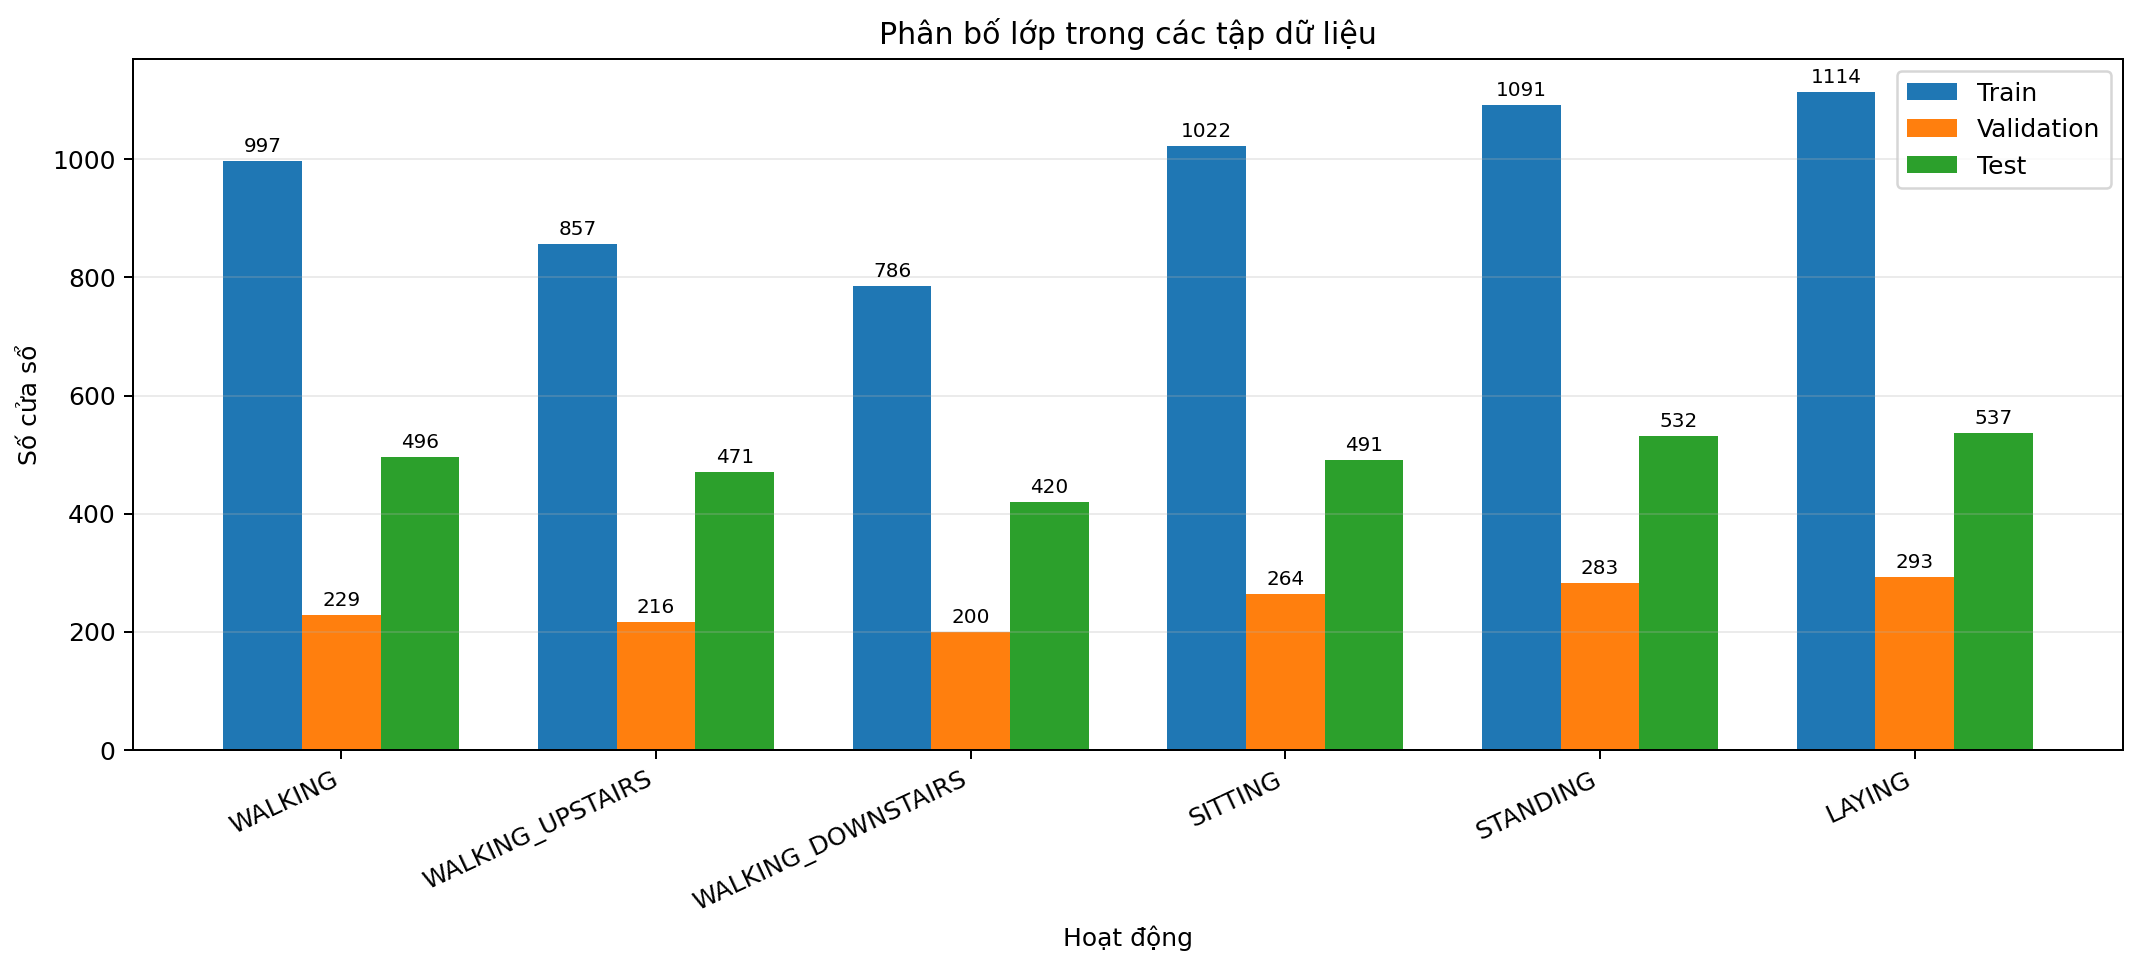
\includegraphics[width=0.92\textwidth]{figures/class_distribution.png}
\caption{Phân bố nhãn theo tập (đầu ra của \code{python main.py visualize-tv1}).}
\label{fig:classdist}
\end{figure}

% =============================== 4. KIẾN TRÚC ===============================
\section{Mô hình ResNetv1-6 một chiều: luồng và thuật toán}

\subsection{Tổng quan}
Mô hình gồm hai khối residual với 32 filter, tiếp theo là GlobalMaxPooling và lớp Dense 6 đầu ra. Tổng cộng $\ParamCount$ tham số, 6 lớp có trọng số. Khối 1 nhận thẳng cửa sổ đã chuẩn hóa (không có lớp stem riêng), đổi $(128,9)\to(64,32)$ và dùng \emph{projection shortcut}; Khối 2 giữ $(64,32)\to(64,32)$ và dùng \emph{identity shortcut}.

\subsection{Luồng xử lý có nhánh}
Hình~\ref{fig:arch} thể hiện luồng suy luận. Có hai \emph{điểm rẽ nhánh}: sau bước chuẩn hóa (vào Khối 1) và sau $x^{(1)}$ (vào Khối 2); mỗi điểm rẽ nhánh cho hai nhánh cùng nguồn, hợp lại tại một node cộng $\oplus$ rồi qua ReLU. Bảng~\ref{tab:branches} liệt kê từng nhánh: bắt đầu từ đâu, đi qua phép toán nào, hợp lại ở đâu.

\begin{figure}[p]
\centering
\begin{tikzpicture}[
  op/.style={draw,rounded corners=2pt,minimum height=8mm,text width=3.3cm,inner sep=2pt,font=\scriptsize,align=center},
  opA/.style={op,fill=blue!10,draw=blue!60!black},
  opB/.style={op,fill=orange!16,draw=orange!70!black},
  opT/.style={op,fill=green!10,draw=green!40!black,text width=5.2cm},
  add/.style={circle,draw,fill=yellow!30,inner sep=1.2pt,font=\small\bfseries},
  arr/.style={-{Stealth[length=1.9mm]},thick},
  arrA/.style={arr,blue!60!black},
  arrB/.style={arr,orange!70!black},
  lab/.style={font=\tiny\itshape,inner sep=1pt}]
\def\xa{-4.1}\def\xb{4.1}
\node[opT] (in) at (0,0) {Cửa sổ cảm biến thô $x^{raw}$\\$(128,9)$};
\node[opT] (zs) at (0,-1.15) {Chuẩn hóa Z-score (N0)\\$x^{n}=(x^{raw}-\mu)/\sigma$};
\node[opA] (a1) at (\xa,-3.5) {N1 Conv1D $K{=}3$, same\\$(128,9)\to(128,32)$};
\node[opA,below=3.2mm of a1] (a2) {N2 ReLU\\$(128,32)$};
\node[opA,below=3.2mm of a2] (a3) {N3 Conv1D $K{=}3$, same\\$(128,32)\to(128,32)$};
\node[opA,below=3.2mm of a3] (a4) {N4 MaxPool /2\\$(128,32)\to(64,32)$};
\node[opB] (b1) at (\xb,-3.5) {N5 Conv1D $K{=}1$ (projection)\\$(128,9)\to(128,32)$};
\node[opB,below=3.2mm of b1] (b2) {N6 MaxPool /2\\$(128,32)\to(64,32)$};
\node[add] (ad1) at (0,-8.05) {$\oplus$};
\node[opT] (r1) at (0,-9.05) {N7+N8 ReLU $\to x^{(1)}$\\$x^{(1)}=\max(0,A+B)$, $(64,32)$};
\node[opA] (c1) at (\xa,-11.8) {N9 Conv1D $K{=}3$, same\\$(64,32)\to(64,32)$};
\node[opA,below=3.2mm of c1] (c2) {N10 ReLU\\$(64,32)$};
\node[opA,below=3.2mm of c2] (c3) {N11 Conv1D $K{=}3$, same\\$(64,32)\to(64,32)$};
\node[opB,dashed] (id) at (\xb,-12.94) {Identity: $S=x^{(1)}$\\không phép toán, không tham số};
\node[add] (ad2) at (0,-15.15) {$\oplus$};
\node[opT] (r2) at (0,-16.15) {N12+N13 ReLU $\to x^{(2)}$\\$x^{(2)}=\max(0,A'+B')$, $(64,32)$};
\node[opT] (gm) at (0,-17.6) {N14 GlobalMaxPool\\$(64,32)\to(32,)$};
\node[opT] (dn) at (0,-18.75) {N15 Dense $32\to6$ (logits thô)\\$z_o=b_o+\sum_i g_iW_{i,o}$};
\node[opT] (am) at (0,-19.9) {argmax $\to$ nhãn $\hat y\in\{0,\dots,5\}$};
\draw[arr] (in)--(zs);
\draw[arrA] (zs.south)--++(0,-4.5mm)-|node[lab,above,pos=.25]{Nhánh A$_1$ (chính)}(a1.north);
\draw[arrB] (zs.south)--++(0,-4.5mm)-|node[lab,above,pos=.25]{Nhánh B$_1$ (shortcut)}(b1.north);
\draw[arrA] (a1)--(a2); \draw[arrA] (a2)--(a3); \draw[arrA] (a3)--(a4);
\draw[arrB] (b1)--(b2);
\draw[arrA] (a4.south)|-node[lab,above,pos=.7]{$A$}(ad1.west);
\draw[arrB] (b2.south)|-node[lab,above,pos=.7]{$B$}(ad1.east);
\draw[arr] (ad1)--(r1);
\draw[arrA] (r1.south)--++(0,-7.5mm)-|node[lab,above,pos=.25]{Nhánh A$_2$ (chính)}(c1.north);
\draw[arrB,dashed] (r1.south)--++(0,-7.5mm)-|node[lab,above,pos=.25]{Nhánh B$_2$ (identity)}(id.north);
\draw[arrA] (c1)--(c2); \draw[arrA] (c2)--(c3);
\draw[arrA] (c3.south)|-node[lab,above,pos=.7]{$A'$}(ad2.west);
\draw[arrB,dashed] (id.south)|-node[lab,above,pos=.7]{$B'$}(ad2.east);
\draw[arr] (ad2)--(r2); \draw[arr] (r2)--(gm); \draw[arr] (gm)--(dn); \draw[arr] (dn)--(am);
\begin{scope}[on background layer]
\node[fit=(a1)(a4)(b1)(ad1)(r1),draw=black!35,dashed,fill=black!3,inner xsep=3mm,inner ysep=3mm,name=blk1] {};
\node[fit=(c1)(c3)(id)(ad2)(r2),draw=black!35,dashed,fill=black!3,inner xsep=3mm,inner ysep=3mm,name=blk2] {};
\node[fit=(gm)(dn)(am),draw=black!35,dashed,fill=black!3,inner sep=3mm,name=blk3] {};
\end{scope}
\node[font=\scriptsize\bfseries,anchor=north] at ($(blk1.north)+(0,-1.5mm)$) {Khối 1: projection shortcut};
\node[font=\scriptsize\bfseries,anchor=north] at ($(blk2.north)+(0,-1.5mm)$) {Khối 2: identity shortcut};
\node[font=\scriptsize\bfseries,anchor=east] at ($(blk3.west)+(-2mm,0)$) {Đầu ra (head)};
\end{tikzpicture}
\caption{Luồng suy luận của ResNetv1-6 một chiều. Màu xanh: nhánh chính A (có trọng số); màu cam: nhánh tắt B (projection ở Khối 1, identity nét đứt ở Khối 2); $\oplus$: điểm hợp nhánh bằng phép cộng phần tử. Nhãn N0--N15 là chỉ số node dùng xuyên suốt tài liệu và mã.}
\label{fig:arch}
\end{figure}

\begin{table}[t]
\centering\footnotesize
\adjustbox{max width=\textwidth}{\begin{tabular}{@{}l l l l l@{}}
\toprule
Nhánh & Xuất phát từ & Phép toán (theo thứ tự) & Hợp lại tại & Shape khi hợp \\
\midrule
A$_1$ (chính, Khối 1) & $x^{n}$ $(128,9)$ & Conv $K{=}3$ $\to$ ReLU $\to$ Conv $K{=}3$ $\to$ MaxPool/2 & $\oplus$ Khối 1 & $(64,32)$ \\
B$_1$ (projection) & $x^{n}$ (cùng nguồn A$_1$) & Conv $K{=}1$ (9$\to$32 kênh) $\to$ MaxPool/2 & $\oplus$ Khối 1 & $(64,32)$ \\
A$_2$ (chính, Khối 2) & $x^{(1)}$ $(64,32)$ & Conv $K{=}3$ $\to$ ReLU $\to$ Conv $K{=}3$ & $\oplus$ Khối 2 & $(64,32)$ \\
B$_2$ (identity) & $x^{(1)}$ (cùng nguồn A$_2$) & không có (truyền thẳng) & $\oplus$ Khối 2 & $(64,32)$ \\
\bottomrule
\end{tabular}}
\caption{Các nhánh của mô hình. Hai nhánh của mỗi khối cùng xuất phát từ \emph{cùng một tensor}, không phải nhánh này nối tiếp nhánh kia.}
\label{tab:branches}
\end{table}

\begin{table}[t]
\centering\scriptsize
\adjustbox{max width=\textwidth}{\begin{tabular}{@{}l l l l r@{}}
\toprule
Node & Phép toán & Công thức & Hàm C (\code{firmware/src/har\_resnet.c}) & Tham số \\
\midrule
N0 & Z-score & Mục~3.3 & \code{har\_normalize} & 18 hằng số \\
N1 & Conv1D $K{=}3$, 9$\to$32 & \eqref{eq:conv}, $p{=}1$ & \code{har\_conv1d\_same} (trong \code{har\_block1\_branch\_main}) & 896 \\
N2 & ReLU & \eqref{eq:relu} & \code{har\_relu} & 0 \\
N3 & Conv1D $K{=}3$, 32$\to$32 & \eqref{eq:conv}, $p{=}1$ & \code{har\_conv1d\_same} (\code{har\_block1\_branch\_main}) & 3.104 \\
N4 & MaxPool/2 & \eqref{eq:pool} & \code{har\_maxpool1d\_2} & 0 \\
N5 & Conv1D $K{=}1$, 9$\to$32 & \eqref{eq:conv}, $p{=}0$ & \code{har\_conv1d\_same} (\code{har\_block1\_branch\_shortcut}) & 320 \\
N6 & MaxPool/2 & \eqref{eq:pool} & \code{har\_maxpool1d\_2} & 0 \\
N7 & Cộng $A+B$ & \eqref{eq:res} & \code{har\_add} (trong \code{har\_residual\_merge\_relu}) & 0 \\
N8 & ReLU sau cộng & \eqref{eq:relu}, \eqref{eq:res} & \code{har\_relu} (\code{har\_residual\_merge\_relu}) & 0 \\
N9 & Conv1D $K{=}3$, 32$\to$32 & \eqref{eq:conv}, $p{=}1$ & \code{har\_conv1d\_same} (\code{har\_block2\_branch\_main}) & 3.104 \\
N10 & ReLU & \eqref{eq:relu} & \code{har\_relu} & 0 \\
N11 & Conv1D $K{=}3$, 32$\to$32 & \eqref{eq:conv}, $p{=}1$ & \code{har\_conv1d\_same} (\code{har\_block2\_branch\_main}) & 3.104 \\
N12 & Cộng $A'+x^{(1)}$ (identity) & \eqref{eq:res} & \code{har\_add} (\code{har\_residual\_merge\_relu}) & 0 \\
N13 & ReLU sau cộng & \eqref{eq:relu}, \eqref{eq:res} & \code{har\_relu} (\code{har\_residual\_merge\_relu}) & 0 \\
N14 & GlobalMaxPool & \eqref{eq:gmp} & \code{har\_global\_max\_pool} (\code{har\_head\_forward}) & 0 \\
N15 & Dense $32\to6$ & \eqref{eq:dense} & \code{har\_dense} (\code{har\_head\_forward}) & 198 \\
-- & argmax & \eqref{eq:dense} & \code{har\_argmax} & 0 \\
\bottomrule
\end{tabular}}
\caption{Ánh xạ từng node của Hình~\ref{fig:arch} sang công thức, hàm C và số tham số. Tổng tham số có trọng số: $896+3.104+320+3.104+3.104+198=\ParamCount$.}
\label{tab:nodemap}
\end{table}

\subsection{Thuật toán từng khối}
Dùng các phép toán \eqref{eq:conv}--\eqref{eq:res}, ký hiệu $\mathrm{Conv}_K(\cdot;W,b)$ là công thức~\eqref{eq:conv} với kernel $K$.

\textbf{Khối 1} (nhận $x^{n}\in\mathbb{R}^{128\times9}$, cho $x^{(1)}\in\mathbb{R}^{64\times32}$):
\begin{align}
A&=\mathrm{MaxPool}_2\Bigl(\mathrm{Conv}_3\bigl(\mathrm{ReLU}(\mathrm{Conv}_3(x^{n};W_1,b_1));W_2,b_2\bigr)\Bigr),\label{eq:A1}\\
B&=\mathrm{MaxPool}_2\bigl(\mathrm{Conv}_1(x^{n};W_p,b_p)\bigr),\label{eq:B1}\\
x^{(1)}&=\mathrm{ReLU}(A+B).\label{eq:x1}
\end{align}

\textbf{Khối 2} (nhận $x^{(1)}$, cho $x^{(2)}\in\mathbb{R}^{64\times32}$):
\begin{align}
A'&=\mathrm{Conv}_3\bigl(\mathrm{ReLU}(\mathrm{Conv}_3(x^{(1)};W_3,b_3));W_4,b_4\bigr),\qquad B'=x^{(1)},\label{eq:A2}\\
x^{(2)}&=\mathrm{ReLU}(A'+B').\label{eq:x2}
\end{align}

\textbf{Đầu ra:} $g=\mathrm{GlobalMaxPool}(x^{(2)})\in\mathbb{R}^{32}$, $z=g\,W_d+b_d\in\mathbb{R}^{6}$ theo \eqref{eq:dense}, $\hat y=\argmax_o z_o$.

\subsection{Số tham số và số phép tính}
Số tham số: Conv1D có $KC_{in}C_{out}+C_{out}$, Dense có $D_{in}D_{out}+D_{out}$. Cộng sáu lớp: $896+3.104+320+3.104+3.104+198=\ParamCount$. Số phép nhân--cộng (MAC) của một lớp Conv1D, có trừ các vị trí kernel rơi ra ngoài biên do zero-padding, là
\begin{equation}
\mathrm{MAC}=\bigl(KL-p(p+1)\bigr)\,C_{in}\,C_{out},
\end{equation}
cho tổng $\MACexact$ MAC mỗi cửa sổ (chặn trên không trừ biên: $\MACupper$).

% =============================== 5. PHƯƠNG PHÁP ===============================
\section{Phương pháp thực nghiệm}

\subsection{Huấn luyện baseline FP32}
Cấu hình bám mục 6.1.1 của bài báo nền (Bảng~\ref{tab:train}). Hàm mất mát là cross-entropy với \code{from\_logits=True}; checkpoint được chọn theo validation accuracy cao nhất. Môi trường: Python 3.10.12, TensorFlow CPU 2.16.1, NumPy 1.26.4, seed 42. Mixup \cite{zhang2018} trộn hai mẫu $(x_i,y_i),(x_j,y_j)$ thành $\lambda x_i+(1-\lambda)x_j$ với nhãn tương ứng, $\lambda\sim\mathrm{Beta}(\alpha,\alpha)$.

\begin{table}[t]
\centering\small
\begin{tabular}{@{}ll@{}}
\toprule
Siêu tham số & Giá trị \\
\midrule
Bộ tối ưu & SGD, momentum 0,9 \\
Batch size / số epoch & 64 / 300 \\
Learning rate ban đầu & 0,05; nhân 0,13 tại epoch 100, 200, 250 \\
Weight decay & $5\times10^{-4}$ \\
Mixup & $\alpha=0{,}2$ (bài báo không công bố $\alpha$) \\
Số filter & 32 \\
\bottomrule
\end{tabular}
\caption{Cấu hình huấn luyện baseline (nguồn: \code{configs/project.json}).}
\label{tab:train}
\end{table}

Các điểm khác bài báo (nêu rõ để không hiểu nhầm là tái hiện nguyên bản): (i) tách subject 27--30 làm validation; (ii) $\alpha=0{,}2$ do bài báo không công bố; (iii) nhánh INT8 là TFLite PTQ thay vì MicroAI/QAT; (iv) kết quả hiện tại là một lần chạy seed 42, còn bài báo báo trung bình 15 lần chạy.

\subsection{PTQ full-integer INT8}
Nguồn mô hình duy nhất là checkpoint FP32 (SHA-256 bắt đầu bằng \code{aa323b3e55d1}; đã kiểm chứng trùng với file thực). Quy trình trong \code{src/quantize.py}:
\begin{enumerate}
  \item Nạp \code{baseline.keras}, kiểm tra SHA-256 với metadata; xuất \code{baseline\_fp32.tflite} để so sánh cùng định dạng file.
  \item Với mỗi kích thước calibration $n\in\{50,200,500\}$ và seed $\{11,22,33\}$, lấy $n$ cửa sổ \emph{không lặp} từ $x_{train}$ (đã Z-score; không chuẩn hóa lại, không dùng validation/test).
  \item Representative dataset cho TFLite Converter quan sát miền giá trị của activation, suy ra $S$ và $Z$ theo \eqref{eq:quant}.
  \item Ép tập toán tử \code{TFLITE\_BUILTINS\_INT8}, đầu vào và đầu ra kiểu \code{int8}.
  \item Mở lại từng mô hình bằng interpreter, kiểm tra mọi tensor; nếu còn tensor float thì dừng thay vì gọi nhầm là full-integer.
\end{enumerate}
Kết quả là một mô hình FP32 TFLite và chín mô hình INT8 ($3\times3$).

\subsection{Quy trình chọn cấu hình và đánh giá}
FP32 và cả chín mô hình INT8 được chạy trên validation; gom ba seed theo từng $n$, chọn $n$ có accuracy trung bình cao nhất (hòa thì ưu tiên macro-F1 trung bình rồi $n$ nhỏ hơn). Chỉ \emph{sau khi chốt $n$} mới mở test và đánh giá FP32 cùng ba seed của $n$ đã chọn. FP32 TFLite và INT8 dùng đúng cùng tensor đã chuẩn hóa, cùng thứ tự nhãn. Cách này tránh dùng test để chọn cấu hình.

\subsection{Trích xuất tham số và sinh mã C}
Lệnh \code{python main.py export-c} (\code{src/export\_c.py}) thực hiện:
\begin{enumerate}
  \item Kiểm tra SHA-256 của \code{baseline.keras} với \code{checkpoint\_id} trong metadata; lệch thì dừng.
  \item Nạp mô hình, lấy trọng số \emph{theo tên layer}, kiểm tra shape từng layer và tổng $=\ParamCount$ khớp \code{model.count\_params()}.
  \item Ghi \code{models/params\_fp32.npz} gồm 14 khóa (mỗi lớp có \code{\_w} và \code{\_b}, cùng \code{input\_mean} và \code{input\_std}) và file \code{params\_manifest.json}.
  \item Sinh mã C tĩnh gồm hai cặp tệp \code{.h} và \code{.c}: \code{har\_resnet\_params} (mảng \code{const float}) và \code{har\_golden} (12 cửa sổ đối chiếu lấy từ \code{sanity\_samples.npz}, kèm logits của Keras).
\end{enumerate}
Quy ước bố cục: tensor kích hoạt \code{[time][channel]}; kernel Conv1D \code{[k][cin][cout]}, đúng thứ tự C-order khi \code{reshape(-1)} mảng Keras, \emph{không transpose}; Dense \code{[din][dout]}. Số thực in dạng \code{\{:.9g\}f} để chuyển float32 sang văn bản rồi đọc lại không mất bit. Lệnh \code{python main.py describe-params} sinh \code{results/parameters\_reference.md} mô tả từng tham số (vai trò, nhánh, shape từng chiều, công thức, tên biến C, thống kê).

\subsection{Cài đặt suy luận bằng C99}
\code{firmware/src/har\_resnet.c} viết tay theo công thức ở Mục~2: sáu hàm phép toán (\code{har\_conv1d\_same}, \code{har\_relu}, \code{har\_maxpool1d\_2}, \code{har\_add}, \code{har\_global\_max\_pool}, \code{har\_dense}) và ba hàm theo khối \code{har\_block1\_forward}, \code{har\_block2\_forward}, \code{har\_head\_forward}, ánh xạ 1--1 với Hình~\ref{fig:arch}. Mã không dùng \code{malloc}, mảng độ dài biến (VLA) hay \code{double}; biên dịch C99 với \code{-Wall -Wextra -Wpedantic} không cảnh báo. Toàn bộ buffer trung gian là năm mảng \code{static float}: hai mảng $128\times32$ và ba mảng $64\times32$ ($57.344$ byte). Do dùng buffer tĩnh, hàm \emph{không an toàn đa luồng}: chỉ một lời gọi suy luận chạy tại một thời điểm.

\lstinputlisting[style=cstyle,caption={Phép Conv1D same trong \code{har\_resnet.c} (đã lược bớt chú thích tiếng Việt).},label=lst:conv]{generated/c_conv1d.c}
\lstinputlisting[style=cstyle,caption={Ba hàm khối và hàm suy luận (đã lược bớt chú thích tiếng Việt). Hàm \code{har\_resnet\_predict} gọi tuần tự Khối 1, Khối 2, Head trên cùng năm buffer tĩnh.},label=lst:blocks]{generated/c_blocks.c}

% =============================== 6. KẾT QUẢ ===============================
\section{Kết quả và thảo luận}

\subsection{Baseline FP32}
Checkpoint được chọn ở epoch $\BestEpoch/300$: train accuracy $\TrainAccBest\%$, validation accuracy $\ValAccBest\%$. Trên test chính thức baseline đạt accuracy $\TestAccFPlong\%$ và macro-F1 $\TestFoneFP$ ($\TestCorrectFP/\TestN$ mẫu đúng). Validation accuracy ở epoch 300 là $\ValAccLast\%$, thấp hơn mức $\ValAccBest\%$ của checkpoint được chọn, nên chọn theo validation là hợp lý; đồng thời vì checkpoint được chọn chính bằng validation, con số validation là ước lượng lạc quan và test mới là con số báo cáo (Hình~\ref{fig:curves}). Dung lượng \code{baseline.keras} là $\KerasBytes$ byte.

\begin{figure}[t]
\centering
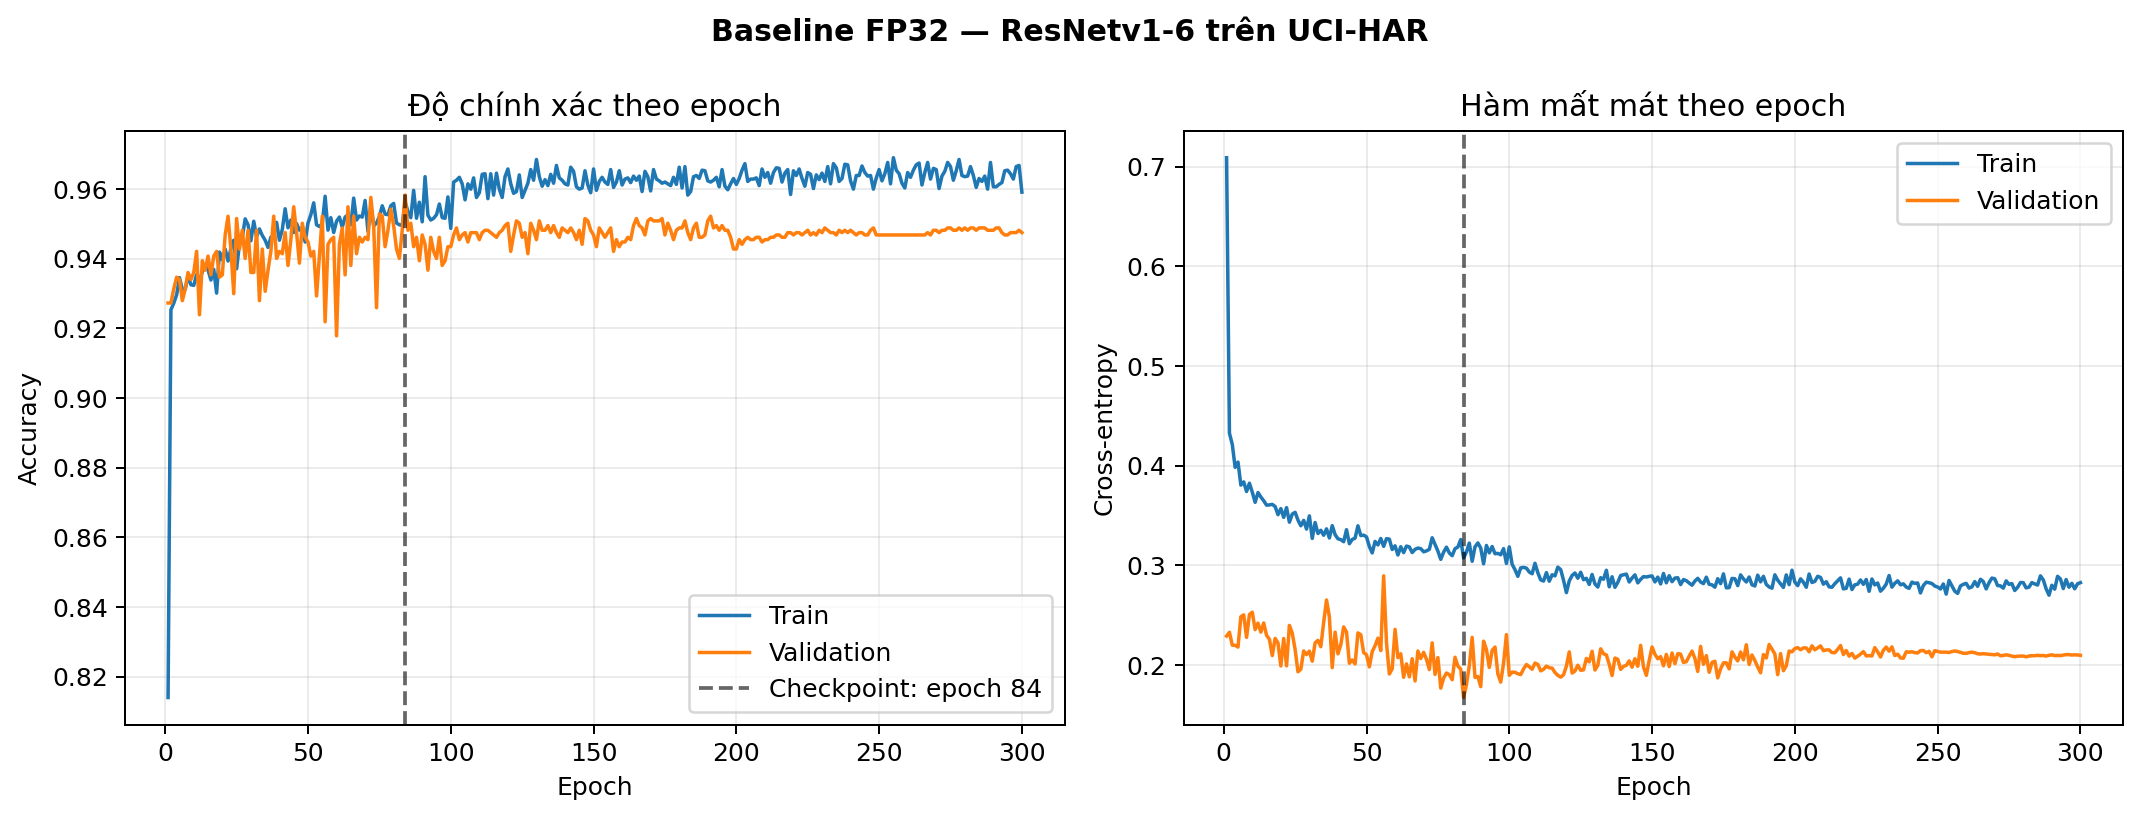
\includegraphics[width=\textwidth]{figures/training_curves.png}
\caption{Accuracy và loss theo epoch của baseline; đường nét đứt đánh dấu checkpoint ở epoch $\BestEpoch$. Learning rate giảm tại epoch 100, 200, 250.}
\label{fig:curves}
\end{figure}

\subsection{Ảnh hưởng của kích thước calibration (validation)}
Bảng~\ref{tab:val} và Hình~\ref{fig:cal} cho thấy accuracy trung bình tăng nhẹ theo $n$ (từ $95{,}6678\%$ lên $95{,}7576\%$) và $n=500$ được chọn. Tuy nhiên chênh lệch giữa ba cấu hình nhỏ hơn độ lệch chuẩn giữa các seed ($0{,}10$--$0{,}18$ điểm \%), nên kết luận phù hợp là $n=500$ tốt nhất \emph{trong phạm vi ba seed đã chạy}, không khẳng định luôn tốt nhất. Đáng chú ý, ở $n=50$ seed 33 cho validation accuracy $95{,}8249\%$, trùng đúng FP32; biến thiên giữa các seed (Bảng~\ref{tab:seed}) vì vậy lớn hơn tác động trung bình của $n$.

\begin{table}[t]
\centering\small
\begin{tabular}{lrrrr}
\toprule
Mô hình & Số lần chạy & Accuracy (\%) & Macro-F1 & Dung lượng (byte) \\
\midrule
FP32 (TFLite) & 1 & 95,8249 & 0,9621 & 51.728 \\
INT8, $n=50$ & 3 & 95,6678 $\pm$ 0,1695 & 0,9607 $\pm$ 0,0015 & 25.104 \\
INT8, $n=200$ & 3 & 95,7127 $\pm$ 0,1029 & 0,9611 $\pm$ 0,0009 & 25.104 \\
INT8, $n=500$ & 3 & \textbf{95,7576 $\pm$ 0,1782} & \textbf{0,9614 $\pm$ 0,0016} & 25.104 \\
\bottomrule
\end{tabular}

\caption{Kết quả validation, trung bình $\pm$ độ lệch chuẩn mẫu qua ba seed (in đậm: cấu hình được chọn).}
\label{tab:val}
\end{table}

\begin{figure}[t]
\centering
\begin{minipage}{0.49\textwidth}\centering
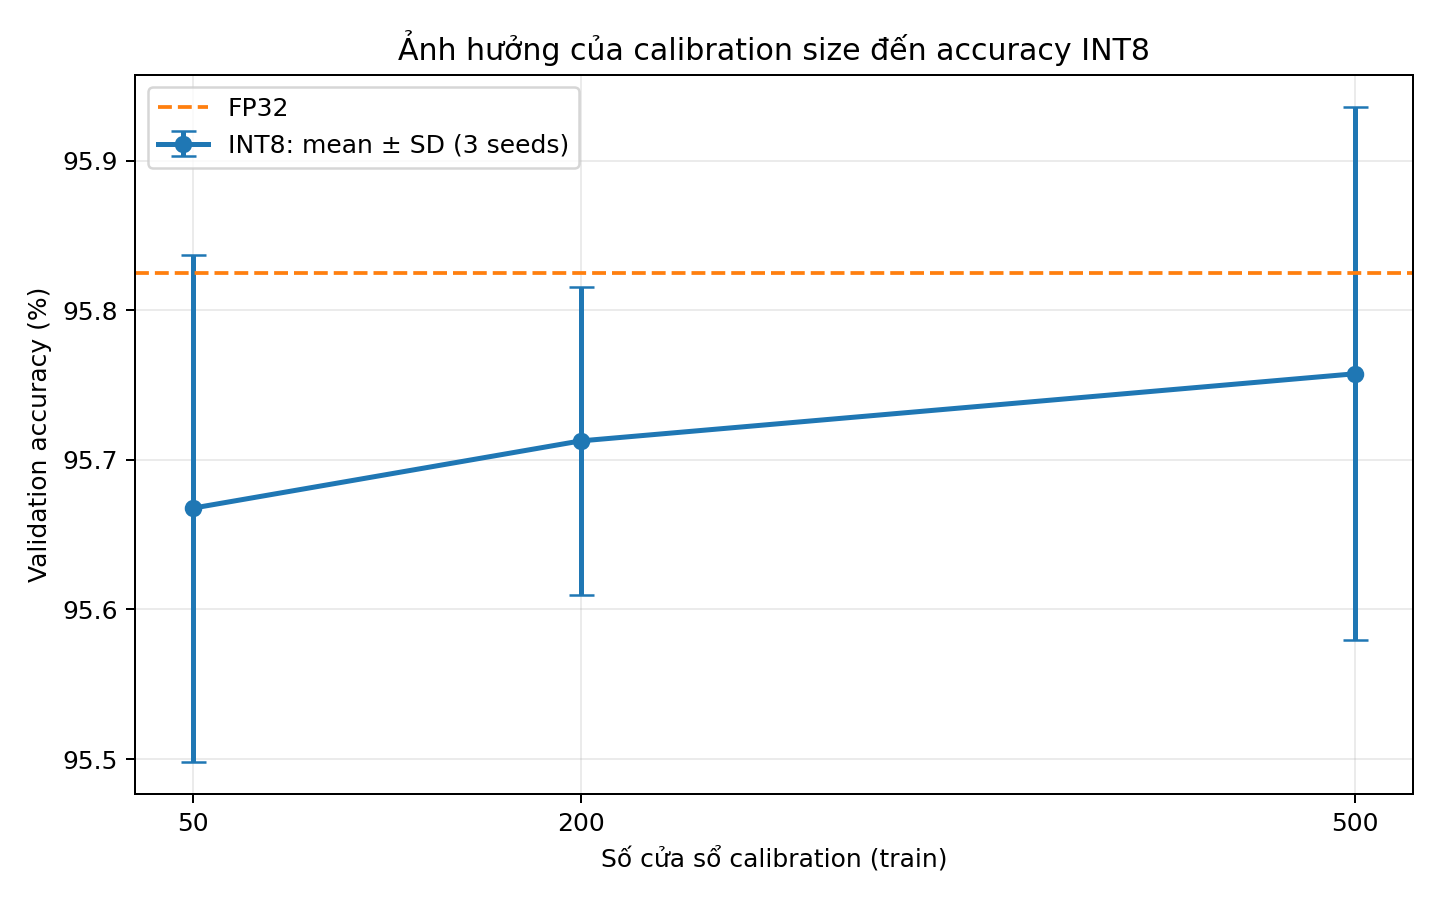
\includegraphics[width=\textwidth]{figures/accuracy_vs_calibration.png}
\end{minipage}\hfill
\begin{minipage}{0.49\textwidth}\centering
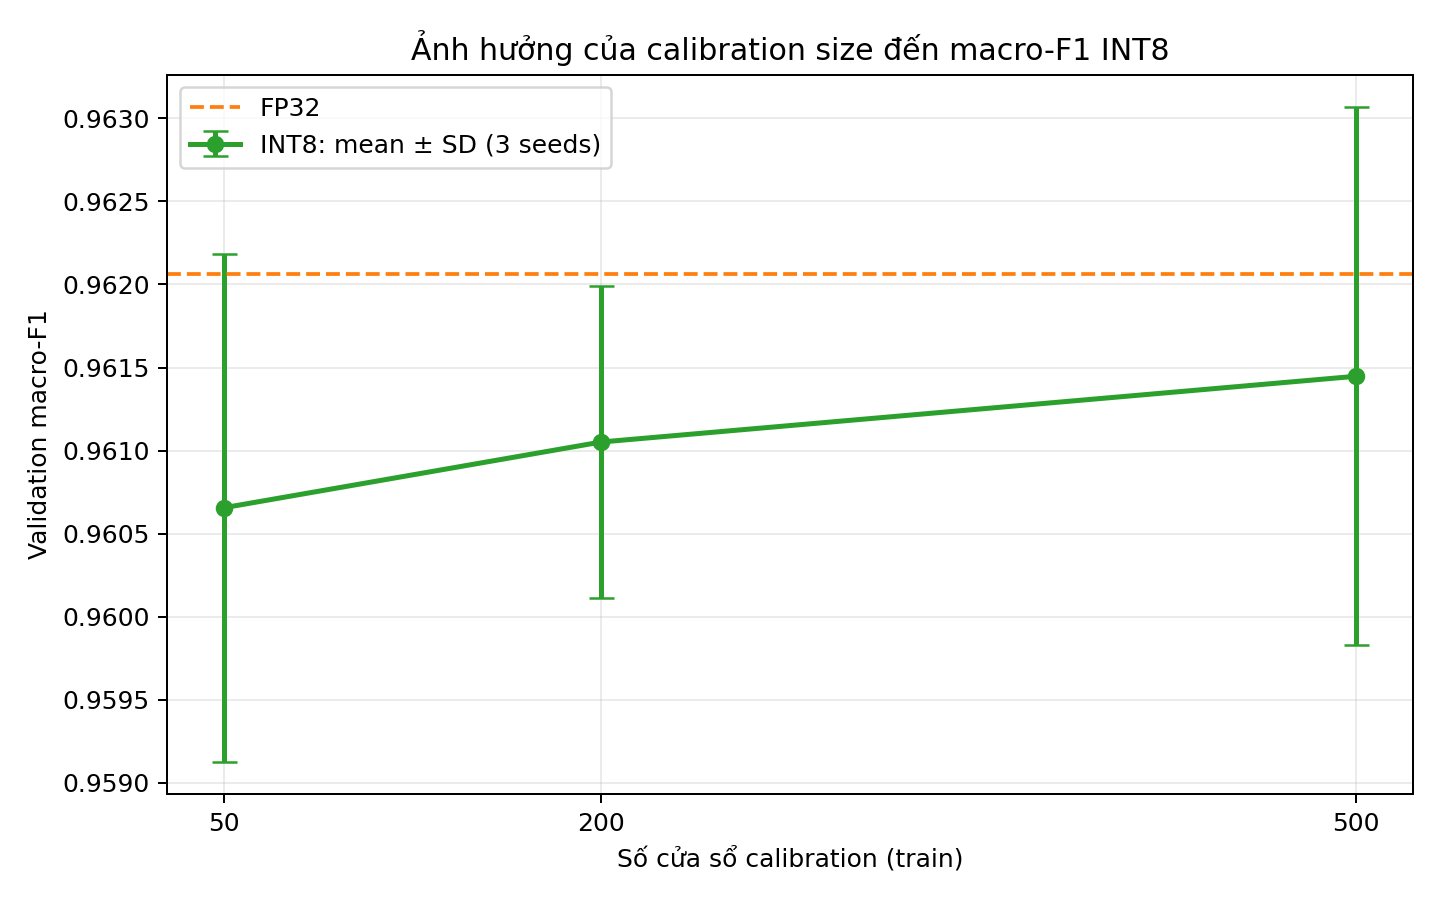
\includegraphics[width=\textwidth]{figures/macro_f1_vs_calibration.png}
\end{minipage}
\caption{Validation accuracy (trái) và macro-F1 (phải) của INT8 theo số cửa sổ calibration; đường nét đứt là FP32, thanh sai số là độ lệch chuẩn qua ba seed.}
\label{fig:cal}
\end{figure}

\subsection{So sánh FP32 và INT8 trên test}
Bảng~\ref{tab:test} là kết quả cuối cùng, đo sau khi chốt $n=500$. INT8 đạt $\TestAccIntlong\pm\TestAccIntSD\%$ và macro-F1 $\TestFoneInt$, thấp hơn FP32 $\TestDelta$ điểm \% accuracy; số mẫu sai tăng từ $\TestErrFP$ (FP32) lên $\TestErrIntMin$--$\TestErrIntMax$ (INT8), tức thêm $\TestErrDiffMin$ đến $\TestErrDiffMax$ mẫu trên $\TestN$ (Bảng~\ref{tab:seed}). FP32 và INT8 được đánh giá trên cùng tập test, nên kiểm định ghép cặp trên dự đoán từng mẫu (ví dụ McNemar) mới cho kết luận chặt chẽ về ý nghĩa thống kê; kho kết quả hiện chỉ lưu ma trận nhầm lẫn nên nhóm chưa thực hiện. Để lấy thang so sánh, độ bất định lấy mẫu nhị thức của chính con số accuracy FP32 trên $\TestN$ mẫu cỡ $\pm\TestSE$ điểm \%, lớn hơn mức giảm trung bình $\TestDeltaShort$ điểm \%.

\begin{table}[t]
\centering\footnotesize
\adjustbox{max width=\textwidth}{\begin{tabular}{lrrrr}
\toprule
Mô hình & Accuracy (\%) & $\Delta$ so với FP32 (điểm \%) & Macro-F1 & Dung lượng (byte) \\
\midrule
FP32 (TFLite) & 92,6026 & 0,0000 & 0,9271 & 51.728 \\
INT8, $n=500$ (3 seed) & 92,1841 $\pm$ 0,2722 & $-$0,4185 & 0,9232 $\pm$ 0,0026 & 25.104 \\
\bottomrule
\end{tabular}
}
\caption{Kết quả test: FP32 TFLite và INT8 $n=500$ (trung bình $\pm$ độ lệch chuẩn qua 3 seed).}
\label{tab:test}
\end{table}

\begin{table}[t]
\centering\footnotesize
\adjustbox{max width=\textwidth}{\begin{tabular}{llrrrrr}
\toprule
Tập & Mô hình & Seed & Accuracy (\%) & Macro-F1 & Số mẫu đúng & Số mẫu sai \\
\midrule
Validation & FP32 & -- & 95,8249 & 0,9621 & 1.423 & 62 \\
Validation & INT8 $n=50$ & 11 & 95,6902 & 0,9609 & 1.421 & 64 \\
Validation & INT8 $n=50$ & 22 & 95,4882 & 0,9590 & 1.418 & 67 \\
Validation & INT8 $n=50$ & 33 & 95,8249 & 0,9621 & 1.423 & 62 \\
Validation & INT8 $n=200$ & 11 & 95,8249 & 0,9621 & 1.423 & 62 \\
Validation & INT8 $n=200$ & 22 & 95,6902 & 0,9608 & 1.421 & 64 \\
Validation & INT8 $n=200$ & 33 & 95,6229 & 0,9602 & 1.420 & 65 \\
Validation & INT8 $n=500$ & 11 & 95,6229 & 0,9602 & 1.420 & 65 \\
Validation & INT8 $n=500$ & 22 & 95,9596 & 0,9633 & 1.425 & 60 \\
Validation & INT8 $n=500$ & 33 & 95,6902 & 0,9608 & 1.421 & 64 \\
\midrule
Test & FP32 & -- & 92,6026 & 0,9271 & 2.729 & 218 \\
Test & INT8 $n=500$ & 11 & 91,9240 & 0,9208 & 2.709 & 238 \\
Test & INT8 $n=500$ & 22 & 92,4669 & 0,9259 & 2.725 & 222 \\
Test & INT8 $n=500$ & 33 & 92,1615 & 0,9228 & 2.716 & 231 \\
\bottomrule
\end{tabular}
}
\caption{Kết quả từng mô hình và từng seed (nguồn: \code{results/metrics.csv}); số mẫu đúng suy ra từ accuracy.}
\label{tab:seed}
\end{table}

\textbf{Theo từng lớp.} Bảng~\ref{tab:perclass} và Hình~\ref{fig:cm} cho thấy lỗi tập trung ở cặp hoạt động tĩnh \code{SITTING}/\code{STANDING}: ở FP32, hai chiều nhầm lẫn này chiếm $\StaticSubjectErrFP$ trên $\TestErrFP$ mẫu sai ($\StaticShareFP\%$). Lượng tử hóa làm giảm recall của hai lớp này nhiều nhất (\code{STANDING} $-1{,}50$ và \code{SITTING} $-1{,}09$ điểm \%), trong khi các lớp chuyển động và \code{LAYING} gần như không đổi. Điều này phù hợp với hai hoạt động tĩnh có tín hiệu quán tính rất giống nhau, vốn đã là điểm khó của FP32; lượng tử hóa không đổi bản chất điểm khó mà làm nó nặng thêm một chút (Bảng~\ref{tab:cmpair}).

\begin{table}[t]
\centering\scriptsize
\adjustbox{max width=\textwidth}{\begin{tabular}{lrrrrrr}
\toprule
Lớp & Số mẫu & Recall FP32 & Recall INT8 & Precision FP32 & Precision INT8 & $\Delta$ recall (điểm \%) \\
\midrule
\texttt{WALKING} & 496 & 95,56 & 95,50 & 95,95 & 95,95 & $-$0,07 \\
\texttt{WALKING\_UPSTAIRS} & 471 & 92,57 & 92,92 & 98,42 & 98,43 & $+$0,35 \\
\texttt{WALKING\_DOWNSTAIRS} & 420 & 95,95 & 96,03 & 95,27 & 95,13 & $+$0,08 \\
\texttt{SITTING} & 491 & 82,89 & 81,81 & 83,06 & 81,92 & $-$1,09 \\
\texttt{STANDING} & 532 & 90,23 & 88,72 & 84,66 & 83,55 & $-$1,50 \\
\texttt{LAYING} & 537 & 98,51 & 98,39 & 99,81 & 99,81 & $-$0,12 \\
\bottomrule
\end{tabular}
}
\caption{Recall và precision theo lớp trên test; INT8 là trung bình ba seed ($n=500$).}
\label{tab:perclass}
\end{table}

\begin{table}[t]
\centering\footnotesize
\begin{tabular}{lrrr}
\toprule
Mô hình & \texttt{SITTING}$\to$\texttt{STANDING} & \texttt{STANDING}$\to$\texttt{SITTING} & Tổng số mẫu sai \\
\midrule
FP32 & 80 & 51 & 218 \\
INT8 $n=500$, seed 11 & 89 & 59 & 238 \\
INT8 $n=500$, seed 22 & 80 & 58 & 222 \\
INT8 $n=500$, seed 33 & 87 & 60 & 231 \\
\bottomrule
\end{tabular}

\caption{Số mẫu bị nhầm giữa \code{SITTING} và \code{STANDING} trên test (hàng: nhãn thật).}
\label{tab:cmpair}
\end{table}

\begin{figure}[t]
\centering
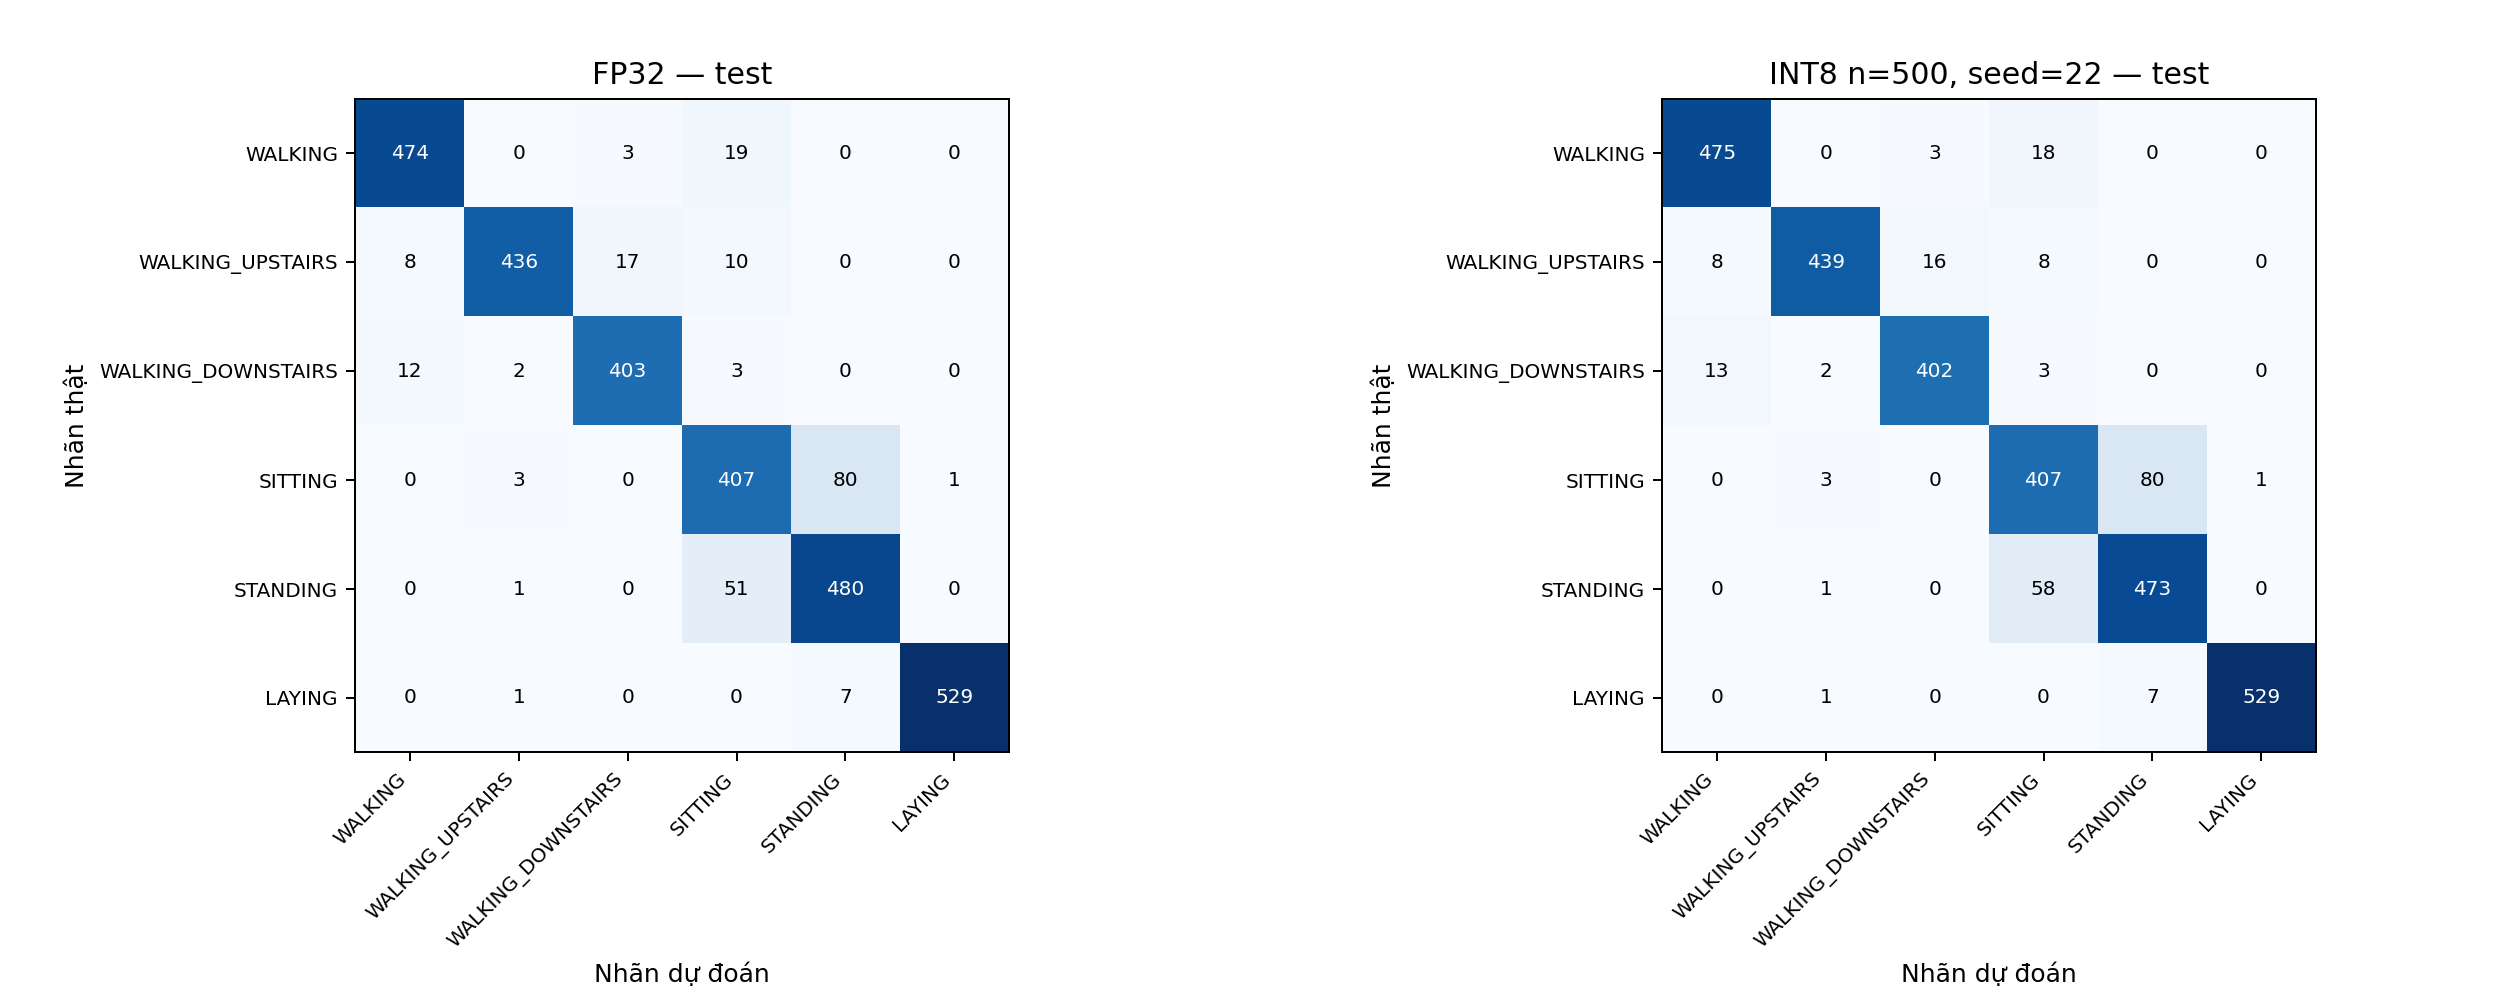
\includegraphics[width=\textwidth]{figures/confusion_matrix_test.png}
\caption{Ma trận nhầm lẫn trên test: FP32 (trái) và INT8 $n=500$, seed 22 (phải, mô hình đại diện được chọn trong \code{results/selection.json}).}
\label{fig:cm}
\end{figure}

\subsection{Dung lượng mô hình}
File FP32 TFLite là $\TfliteFP$ byte, INT8 là $\TfliteInt$ byte (cả chín mô hình INT8 bằng nhau), giảm $\SizeRed\%$, hệ số nén $\SizeRatio$ lần (Hình~\ref{fig:size}). Con số này \emph{không} đạt bốn lần dù trọng số xuống 8 bit, vì mạng nhỏ và file còn chứa đồ thị, shape, tham số lượng tử và metadata cố định. Cụ thể, riêng trọng số FP32 là $\ParamCount\times4=\ParamBytesFP$ byte, còn INT8 là $\ParamBytesInt$ byte (đúng bốn lần); phần còn lại trong file là $\TfliteFP-\ParamBytesFP=8.824$ byte (FP32) và $\TfliteInt-\ParamBytesInt=14.378$ byte (INT8). Phần dư lớn hơn ở INT8 phù hợp với việc mỗi tensor lượng tử hóa mang thêm scale/zero-point (theo kênh với trọng số) và bias lưu 32 bit; nhóm không phân rã chính xác từng byte của file. Mô hình INT8 gồm 23 toán tử (5 \code{CONV\_2D}, 2 \code{MAX\_POOL\_2D}, 2 \code{ADD}, 1 \code{REDUCE\_MAX}, 1 \code{FULLY\_CONNECTED}, cùng 6 \code{EXPAND\_DIMS} và 6 \code{RESHAPE}, nghĩa là Conv1D được hiện thực bằng Conv2D); ReLU không xuất hiện thành toán tử riêng, thường do TFLite gộp vào toán tử đứng trước. Đây là dung lượng file, không phải Flash/RAM thực đo trên vi điều khiển.

\begin{figure}[t]
\centering
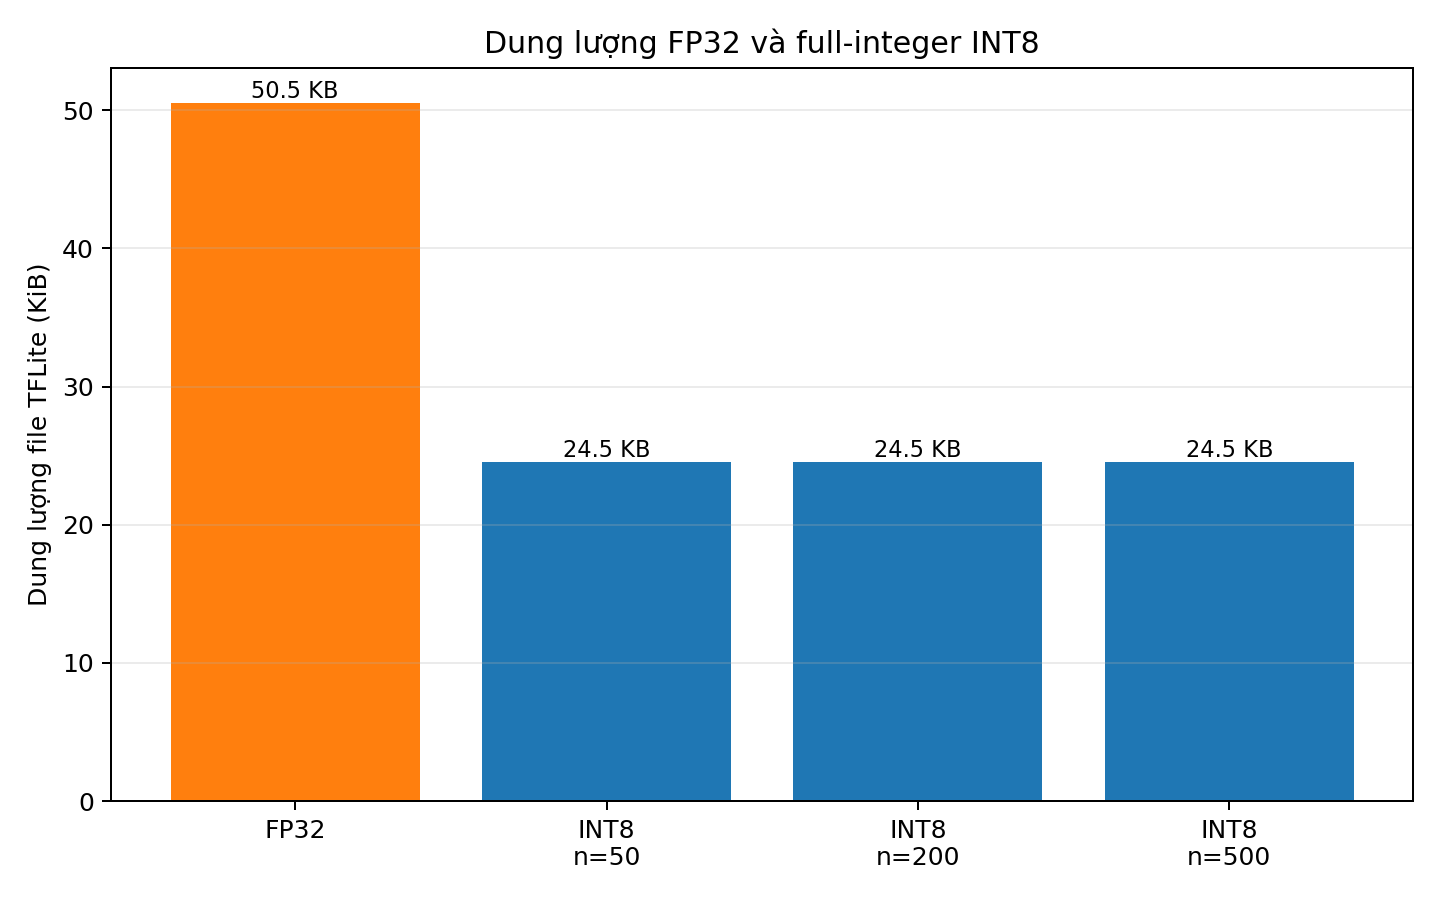
\includegraphics[width=0.62\textwidth]{figures/model_size_comparison.png}
\caption{Dung lượng file TFLite: FP32 và INT8 với ba kích thước calibration.}
\label{fig:size}
\end{figure}

\subsection{Kết quả trích xuất tham số}
Từ checkpoint FP32, \code{export-c} trích đủ $\ParamCount$ tham số; Bảng~\ref{tab:poverview} cho cấu trúc, Bảng~\ref{tab:pstats} cho thống kê, và các bảng sau đưa ra giá trị cụ thể của một số tensor. Toàn bộ thống kê được tính lại từ \code{params\_fp32.npz} và khớp \code{results/parameters\_reference.md}.

\begin{table}[t]
\centering\scriptsize
\adjustbox{max width=\textwidth}{\begin{tabular}{rllllrrr}
\toprule
\# & Layer & Khối & Nhánh & Phép toán & Shape kernel & Số tham số & \% tổng \\
\midrule
1 & \texttt{block1\_conv1} & Khối 1 & A (chính) & Conv1D, $K{=}3$, same & (3, 9, 32) & 896 & 8,35 \\
2 & \texttt{block1\_conv2} & Khối 1 & A (chính) & Conv1D, $K{=}3$, same & (3, 32, 32) & 3.104 & 28,94 \\
3 & \texttt{block1\_projection} & Khối 1 & B (shortcut) & Conv1D, $K{=}1$, valid & (1, 9, 32) & 320 & 2,98 \\
4 & \texttt{block2\_conv1} & Khối 2 & A (chính) & Conv1D, $K{=}3$, same & (3, 32, 32) & 3.104 & 28,94 \\
5 & \texttt{block2\_conv2} & Khối 2 & A (chính) & Conv1D, $K{=}3$, same & (3, 32, 32) & 3.104 & 28,94 \\
6 & \texttt{activity\_logits} & Đầu ra & -- & Dense $32\to6$ & (32, 6) & 198 & 1,85 \\
\midrule
& & & & & \textbf{Tổng} & \textbf{10.726} & \textbf{100,00} \\
\bottomrule
\end{tabular}
}
\caption{Tham số đã trích xuất theo layer. Bốn lớp Conv $K{=}3$ ở nhánh chính chiếm $95{,}17\%$ tổng tham số; lớp chiếu nhánh B chỉ $2{,}98\%$ và lớp Dense $1{,}85\%$.}
\label{tab:poverview}
\end{table}

\begin{table}[t]
\centering\scriptsize
\adjustbox{max width=\textwidth}{\begin{tabular}{llrrrrr}
\toprule
Layer & Tensor & Số phần tử & min & max & trung bình & độ lệch chuẩn \\
\midrule
\texttt{block1\_conv1} & kernel & 864 & $-$0,7666 & $+$0,7822 & $+$0,0014 & 0,2509 \\
 & bias & 32 & $-$0,8689 & $+$0,5869 & $-$0,1822 & 0,3396 \\
\addlinespace[2pt]
\texttt{block1\_conv2} & kernel & 3.072 & $-$0,6782 & $+$0,4601 & $-$0,0376 & 0,1425 \\
 & bias & 32 & $-$0,8619 & $+$0,6701 & $+$0,0708 & 0,2806 \\
\addlinespace[2pt]
\texttt{block1\_projection} & kernel & 288 & $-$1,0266 & $+$1,2403 & $+$0,0169 & 0,3021 \\
 & bias & 32 & $-$0,8619 & $+$0,6701 & $+$0,0708 & 0,2806 \\
\addlinespace[2pt]
\texttt{block2\_conv1} & kernel & 3.072 & $-$0,5980 & $+$0,5741 & $-$0,0244 & 0,1439 \\
 & bias & 32 & $-$0,5400 & $+$0,5516 & $-$0,0289 & 0,2893 \\
\addlinespace[2pt]
\texttt{block2\_conv2} & kernel & 3.072 & $-$0,5754 & $+$0,5147 & $-$0,0257 & 0,1335 \\
 & bias & 32 & $-$0,5410 & $+$1,2143 & $-$0,0412 & 0,3124 \\
\addlinespace[2pt]
\texttt{activity\_logits} & kernel & 192 & $-$1,3688 & $+$0,9113 & $+$0,0186 & 0,3290 \\
 & bias & 6 & $-$1,0907 & $+$1,3195 & 0,0000 & 1,0229 \\
\bottomrule
\end{tabular}
}
\caption{Thống kê số học của từng tensor (kernel, bias). Không có trọng số bằng đúng 0 ở layer nào.}
\label{tab:pstats}
\end{table}

\textbf{Tham số chuẩn hóa đầu vào.} Bảng~\ref{tab:zscore} liệt kê $\mu_c,\sigma_c$ của chín kênh, được nhúng vào mã C (\code{har\_input\_mean}, \code{har\_input\_std}). Kênh gia tốc tổng theo trục $x$ có trung bình $\approx0{,}81$ vì chứa thành phần trọng lực, còn các kênh \code{body\_*} có trung bình gần 0.

\begin{table}[t]
\centering\small
\begin{tabular}{rlrr}
\toprule
\# & Kênh & $\mu_c$ & $\sigma_c$ \\
\midrule
0 & \texttt{total\_acc\_x} & $+$0,805391 & 0,410322 \\
1 & \texttt{total\_acc\_y} & $+$0,029006 & 0,399567 \\
2 & \texttt{total\_acc\_z} & $+$0,080120 & 0,354005 \\
3 & \texttt{body\_gyro\_x} & $+$0,004766 & 0,408725 \\
4 & \texttt{body\_gyro\_y} & $-$0,002092 & 0,382862 \\
5 & \texttt{body\_gyro\_z} & $-$0,000882 & 0,258296 \\
6 & \texttt{body\_acc\_x} & $-$0,000794 & 0,197001 \\
7 & \texttt{body\_acc\_y} & $-$0,000252 & 0,126466 \\
8 & \texttt{body\_acc\_z} & $-$0,000306 & 0,108309 \\
\bottomrule
\end{tabular}

\caption{Tham số Z-score theo kênh (fit trên tập train mô hình).}
\label{tab:zscore}
\end{table}

\textbf{Trọng số lớp phân loại.} Bảng~\ref{tab:dense} là toàn bộ $32\times6+6=198$ tham số của \code{activity\_logits}: cột $o$ là trọng số nối 32 đặc trưng sau GlobalMaxPool tới logit của lớp thứ $o$; hàng cuối là bias.

\begin{table}[t]
\centering\scriptsize
\adjustbox{max width=\textwidth}{\begin{tabular}{rrrrrrr}
\toprule
$i$ & $W_{i,0}$ (WALK) & $W_{i,1}$ (UP) & $W_{i,2}$ (DOWN) & $W_{i,3}$ (SIT) & $W_{i,4}$ (STAND) & $W_{i,5}$ (LAY) \\
\midrule
0 & $+$0,1220 & $-$0,1532 & $+$0,1674 & $-$0,1572 & $+$0,5603 & $-$0,2510 \\
1 & $+$0,2476 & $+$0,5378 & $+$0,0287 & $-$0,1578 & $+$0,2236 & $+$0,1310 \\
2 & $-$0,1774 & $-$0,3461 & $+$0,5742 & $-$0,2613 & $-$0,1697 & $-$0,0609 \\
3 & $+$0,6200 & $-$0,1224 & $-$0,0557 & $-$0,1071 & $-$0,1122 & $+$0,1811 \\
4 & $+$0,0218 & $+$0,5228 & $+$0,1563 & $+$0,0911 & $+$0,0705 & $+$0,1851 \\
5 & $+$0,0747 & $-$0,0015 & $+$0,0163 & $+$0,6488 & $-$0,2407 & $-$0,1888 \\
6 & $+$0,2125 & $-$0,2097 & $-$0,1106 & $-$0,1618 & $-$0,3441 & $-$0,1183 \\
7 & $+$0,3183 & $+$0,1543 & $+$0,2512 & $-$0,0529 & $+$0,3270 & $+$0,0025 \\
8 & $+$0,1319 & $-$0,1722 & $+$0,1796 & $+$0,0068 & $-$0,2766 & $+$0,0082 \\
9 & $+$0,1553 & $-$0,2212 & $+$0,1969 & $+$0,2753 & $+$0,1306 & $+$0,1299 \\
10 & $+$0,5160 & $+$0,3572 & $+$0,1914 & $+$0,2755 & $+$0,6152 & $-$1,3688 \\
11 & $+$0,0489 & $-$0,4124 & $-$0,2870 & $+$0,4899 & $+$0,1995 & $-$0,0337 \\
12 & $-$0,0392 & $+$0,2016 & $-$0,0930 & $-$0,4065 & $+$0,4382 & $-$0,0663 \\
13 & $+$0,2244 & $-$0,0893 & $+$0,1855 & $-$0,2424 & $+$0,5357 & $-$0,4969 \\
14 & $+$0,2307 & $+$0,1067 & $+$0,0512 & $+$0,3517 & $-$0,4180 & $+$0,1631 \\
15 & $-$0,2092 & $-$0,1823 & $+$0,0260 & $-$0,0572 & $-$0,3345 & $+$0,9113 \\
16 & $-$0,2471 & $-$0,1259 & $-$0,1040 & $+$0,6953 & $+$0,0535 & $+$0,0012 \\
17 & $-$0,1196 & $+$0,0813 & $+$0,0173 & $+$0,2682 & $-$0,6713 & $-$0,2553 \\
18 & $-$0,5144 & $-$0,4805 & $-$0,6201 & $+$0,7217 & $+$0,6369 & $+$0,2566 \\
19 & $-$0,1813 & $-$0,0103 & $-$0,0919 & $-$0,4555 & $+$0,4471 & $+$0,0214 \\
20 & $-$0,2525 & $-$0,3858 & $-$0,0506 & $+$0,5644 & $+$0,1174 & $-$0,2859 \\
21 & $-$0,2676 & $-$0,2568 & $+$0,7880 & $-$0,5745 & $-$0,4911 & $-$0,2306 \\
22 & $+$0,1406 & $+$0,2201 & $+$0,1340 & $-$0,2082 & $-$0,5124 & $+$0,2720 \\
23 & $-$0,2808 & $+$0,5147 & $-$0,1133 & $+$0,0725 & $-$0,3113 & $-$0,0571 \\
24 & $+$0,2401 & $+$0,3392 & $+$0,1145 & $-$0,4053 & $-$0,0572 & $+$0,2075 \\
25 & $+$0,1233 & $+$0,0673 & $+$0,2419 & $-$0,3966 & $-$0,0835 & $-$0,5704 \\
26 & $+$0,1420 & $+$0,2557 & $-$0,0044 & $-$0,3969 & $-$0,2923 & $+$0,1722 \\
27 & $+$0,2526 & $-$0,2549 & $-$0,0944 & $+$0,1491 & $+$0,4079 & $+$0,1172 \\
28 & $+$0,8616 & $+$0,1610 & $-$0,0753 & $-$0,0982 & $-$0,4140 & $-$0,0064 \\
29 & $+$0,0534 & $+$0,4234 & $+$0,4287 & $+$0,0288 & $-$0,2182 & $-$0,8381 \\
30 & $-$0,2320 & $+$0,7949 & $-$0,0168 & $-$0,0004 & $-$0,2621 & $-$0,0957 \\
31 & $+$0,0224 & $+$0,3162 & $+$0,1494 & $-$0,2963 & $+$0,2266 & $-$0,2956 \\
\midrule
$b_o$ & $-$0,9656 & $-$0,8051 & $-$1,0907 & $+$1,3195 & $+$1,3083 & $+$0,2336 \\
\bottomrule
\end{tabular}
}
\caption{Toàn bộ trọng số và bias của lớp \code{activity\_logits} (các cột theo thứ tự nhãn \code{WALKING}, \dots, \code{LAYING}).}
\label{tab:dense}
\end{table}

\textbf{Ví dụ trích từ lớp Conv đầu.} Bảng~\ref{tab:filter0} là kernel của filter đầu tiên (đầu ra $c_o=0$) của \code{block1\_conv1}: ba vị trí thời gian $k$ nhân với chín kênh vào. Kernel đầy đủ của lớp chiếu nhánh B ($1\times9\times32$) nằm ở Phụ lục~\ref{app:proj}.

\begin{table}[t]
\centering\scriptsize
\begin{tabular}{rrrrrrrrrr}
\toprule
$k$ & $c_i{=}0$ & $c_i{=}1$ & $c_i{=}2$ & $c_i{=}3$ & $c_i{=}4$ & $c_i{=}5$ & $c_i{=}6$ & $c_i{=}7$ & $c_i{=}8$ \\
\midrule
0 & $+$0,621 & $-$0,767 & $-$0,058 & $+$0,182 & $+$0,071 & $-$0,111 & $-$0,328 & $-$0,068 & $+$0,165 \\
1 & $+$0,609 & $-$0,649 & $+$0,177 & $-$0,111 & $-$0,024 & $+$0,097 & $-$0,358 & $+$0,234 & $+$0,028 \\
2 & $+$0,443 & $-$0,649 & $+$0,121 & $-$0,302 & $-$0,056 & $+$0,052 & $-$0,098 & $+$0,343 & $-$0,037 \\
\bottomrule
\end{tabular}

\caption{Kernel $W_{k,c_i,0}$ của filter 0 trong \code{block1\_conv1} (hình dạng $3\times9$).}
\label{tab:filter0}
\end{table}

\textbf{Tham số lượng tử hóa INT8.} Ngoài trọng số FP32, mỗi mô hình INT8 mang tham số affine \eqref{eq:quant} cho đầu vào và đầu ra (Bảng~\ref{tab:qio}). Scale và zero-point thay đổi theo tập calibration, nên ba seed cho ba bộ giá trị khác nhau với cùng một checkpoint; đây là nguồn biến thiên của kết quả INT8. Cả chín mô hình đều full-integer (không còn tensor float).

\begin{table}[t]
\centering\scriptsize
\adjustbox{max width=\textwidth}{\begin{tabular}{lrrrrr}
\toprule
Mô hình & Scale vào & Zero-point vào & Scale ra & Zero-point ra & Số tensor float \\
\midrule
INT8 $n=50$, seed 11 & 0.069558 & -6 & 0.048779 & -33 & 0 \\
INT8 $n=50$, seed 22 & 0.065165 & 9 & 0.048235 & -35 & 0 \\
INT8 $n=50$, seed 33 & 0.077086 & 1 & 0.052187 & -28 & 0 \\
INT8 $n=200$, seed 11 & 0.086882 & -26 & 0.052371 & -32 & 0 \\
INT8 $n=200$, seed 22 & 0.088959 & 14 & 0.053451 & -38 & 0 \\
INT8 $n=200$, seed 33 & 0.077859 & 21 & 0.054190 & -46 & 0 \\
INT8 $n=500$, seed 11 & 0.091455 & -2 & 0.054448 & -30 & 0 \\
INT8 $n=500$, seed 22 & 0.087212 & -4 & 0.059316 & -28 & 0 \\
INT8 $n=500$, seed 33 & 0.088829 & 4 & 0.055678 & -27 & 0 \\
\bottomrule
\end{tabular}
}
\caption{Scale và zero-point của đầu vào/đầu ra các mô hình INT8 (nguồn: \code{models/model\_metadata.json}).}
\label{tab:qio}
\end{table}

\textbf{Tệp C sinh tự động và bộ nhớ tham số.} Bảng~\ref{tab:cfiles} cho kích thước và SHA-256 của các tệp C được sinh; đoạn dưới đây là phần đầu của mảng trọng số \code{block1\_conv1} đúng như trong mã (hai dòng giá trị đầu, đối chiếu khớp \code{params\_fp32.npz}). Bộ nhớ tham số lý thuyết là $\ParamBytesFP$ byte ở FP32 và $\ParamBytesInt$ byte nếu mọi tham số lưu 8 bit; con số này khác dung lượng file TFLite đo ở trên.

\begin{table}[t]
\centering\scriptsize
\adjustbox{max width=\textwidth}{\begin{tabular}{lrl}
\toprule
Tệp sinh tự động & Byte & SHA-256 \\
\midrule
\texttt{include/har\_resnet\_params.h} & 2.113 & \texttt{\scriptsize a24805c6ec09515b144d425f1e4fa5d761548f1cf8c499003e4b20506e0dada0} \\
\texttt{src/har\_resnet\_params.c} & 168.839 & \texttt{\scriptsize 75aa6d044e1c3efe9551ceadfe12dadcaccadcd997dc9a7f9769b65596402585} \\
\texttt{include/har\_golden.h} & 537 & \texttt{\scriptsize 871b27be97d60ed8d9dd7e667a22942bcd4b3a574278389e30ff4a65c850e572} \\
\texttt{src/har\_golden.c} & 209.743 & \texttt{\scriptsize 81904accaae525a4290643433c0649d9bec0205e902d538cf821f0102af4345e} \\
\bottomrule
\end{tabular}
}
\caption{Tệp C sinh tự động bởi \code{export-c} (nguồn: \code{models/params\_manifest.json}).}
\label{tab:cfiles}
\end{table}

\lstinputlisting[style=cstylesmall,caption={Đầu mảng \code{har\_block1\_conv1\_w} trong \code{har\_resnet\_params.c}.},label=lst:params]{generated/c_params_excerpt.c}

\subsection{Kết quả suy luận bằng C}
Mã C được đối chiếu với Keras trên 12 cửa sổ validation (hai cửa sổ mỗi lớp) đã lưu cùng logits của Keras:
\begin{itemize}
  \item Tham chiếu NumPy (\code{reference\_forward.py}, cùng thuật toán với C) so với Keras: sai số logits lớn nhất $1{,}9\times10^{-6}$, argmax khớp 12/12.
  \item Chương trình C: argmax khớp 12/12, sai số logits lớn nhất cỡ $10^{-6}$ (ngưỡng chấp nhận $10^{-3}$); hàm \code{har\_normalize} sai số $\le6\times10^{-8}$; kiểm tra ba hàm khối chạy tuần tự so với \code{har\_resnet\_predict} nguyên khối cho kết quả \emph{bằng nhau tuyệt đối}.
  \item Biên dịch C99 \code{-Wall -Wextra -Wpedantic}: 0 cảnh báo. Bộ kiểm thử tự động của repository (\code{python -m pytest -q}) hiện đạt 37/37 test.
  \item Bộ nhớ: buffer trung gian tĩnh $57.344$ byte; cộng đầu vào $4.608$ byte, mảng cục bộ 128 byte và logits 24 byte, RAM hoạt động ước lượng $62.104$ byte; bảng trọng số ($\ParamBytesFP$ byte) là \code{const} nên nằm ở vùng chỉ đọc. Mỗi cửa sổ cần $\MACexact$ phép nhân--cộng.
\end{itemize}
Các con số bộ nhớ và MAC là \emph{ước lượng/đếm theo thiết kế}; chưa đo trên vi điều khiển, và chưa đo accuracy của bản C trên toàn tập test ($\TestN$ cửa sổ).

\subsection{Thảo luận}
\textbf{Đánh đổi.} Với cấu hình khảo sát, PTQ INT8 cho file nhỏ đi hơn một nửa với mức giảm accuracy dưới $0{,}5$ điểm \%, và mức giảm này tập trung vào cặp \code{SITTING}/\code{STANDING}. \textbf{Hệ số nén.} Hệ số $\SizeRatio$ lần thấp hơn mức lý thuyết bốn lần vì phần dư cố định của định dạng file lớn so với mạng chỉ có $\ParamCount$ tham số. \textbf{Độ tin cậy.} Chỉ có một baseline (seed 42), ba seed calibration và một tập test; khác biệt giữa các $n$ nằm trong nhiễu giữa các seed.

\textbf{Giới hạn.} (i) Một kiến trúc, một bộ dữ liệu, ba giá trị $n$. (ii) Không đo độ trễ, RAM, Flash, năng lượng; không suy từ laptop. (iii) Kết quả là TFLite PTQ INT8, không so trực tiếp với MicroAI/QAT của bài báo. (iv) Mã C mới là FP32 tham chiếu; INT8 trong C chưa làm. (v) Chưa có kiểm định thống kê ghép cặp giữa FP32 và INT8.

% =============================== 7. KẾT LUẬN ===============================
\section{Kết luận và hướng phát triển}
Báo cáo đã (1) xây dựng baseline FP32 ResNetv1-6 một chiều trên UCI-HAR đạt $\TestAccFP\%$ accuracy và macro-F1 $\TestFoneFP$ trên test; (2) lượng tử hóa PTQ full-integer INT8, chọn $n=500$ bằng validation, đạt $\TestAccIntlong\pm\TestAccIntSD\%$ trên test với file nhỏ hơn $\SizeRed\%$; (3) mô tả luồng và thuật toán của mô hình theo từng khối và từng nhánh bằng công thức; (4) trích xuất toàn bộ $\ParamCount$ tham số kèm thống kê và giá trị cụ thể; (5) cài đặt suy luận C99 thuần khớp với Keras trên 12 cửa sổ đối chiếu.

\textbf{Hướng phát triển:} cài INT8 trong C (tích lũy \code{int32}, requantize bằng multiplier và shift) và xuất trọng số INT8; port sang vi điều khiển rồi đo RAM, Flash, độ trễ và năng lượng thật; đo accuracy của bản C trên toàn tập test; thử QAT hoặc nhiều seed huấn luyện hơn để so sánh công bằng với bài báo; kiểm định ghép cặp FP32 và INT8.

% =============================== TÀI LIỆU THAM KHẢO ===============================
\begin{thebibliography}{9}
\bibitem{novac2021} P.-E. Novac, G. Boukli Hacene, A. Pegatoquet, B. Miramond, V. Gripon. Quantization and Deployment of Deep Neural Networks on Microcontrollers. \emph{Sensors}, 21(9):2984, 2021. \url{https://doi.org/10.3390/s21092984}
\bibitem{anguita2013} D. Anguita, A. Ghio, L. Oneto, X. Parra, J. L. Reyes-Ortiz. A Public Domain Dataset for Human Activity Recognition Using Smartphones. \emph{ESANN}, 2013. Dữ liệu: \url{https://doi.org/10.24432/C54S4K}
\bibitem{he2016} K. He, X. Zhang, S. Ren, J. Sun. Deep Residual Learning for Image Recognition. \emph{CVPR}, 770--778, 2016.
\bibitem{jacob2018} B. Jacob, S. Kligys, B. Chen, M. Zhu, M. Tang, A. Howard, H. Adam, D. Kalenichenko. Quantization and Training of Neural Networks for Efficient Integer-Arithmetic-Only Inference. \emph{CVPR}, 2704--2713, 2018.
\bibitem{krishnamoorthi2018} R. Krishnamoorthi. Quantizing deep convolutional networks for efficient inference: A whitepaper. \emph{arXiv:1806.08342}, 2018.
\bibitem{zhang2018} H. Zhang, M. Cisse, Y. N. Dauphin, D. Lopez-Paz. mixup: Beyond Empirical Risk Minimization. \emph{ICLR}, 2018.
\end{thebibliography}

% =============================== PHỤ LỤC ===============================
\appendix
\section{Kernel đầy đủ của lớp chiếu nhánh B}\label{app:proj}
Bảng~\ref{tab:proj} là toàn bộ $1\times9\times32+32=320$ tham số của \code{block1\_projection} (Conv1D $K=1$, đổi 9 kênh cảm biến thành 32 kênh): hàng $c_o$ là một filter, các cột $c_i$ là trọng số tương ứng chín kênh vào theo thứ tự \code{total\_acc\_x}, \dots, \code{body\_acc\_z}; cột cuối là bias.

\begin{table}[h]
\centering\scriptsize
\adjustbox{max width=\textwidth}{\begin{tabular}{rrrrrrrrrrr}
\toprule
$c_o$ & $c_i{=}0$ & $c_i{=}1$ & $c_i{=}2$ & $c_i{=}3$ & $c_i{=}4$ & $c_i{=}5$ & $c_i{=}6$ & $c_i{=}7$ & $c_i{=}8$ & $b$ \\
\midrule
0 & $+$0,879 & $-$0,538 & $-$0,510 & $-$0,725 & $-$0,141 & $-$0,242 & $-$0,416 & $+$0,111 & $+$0,198 & $-$0,143 \\
1 & $-$0,294 & $+$0,340 & $-$0,121 & $+$0,409 & $-$0,040 & $-$0,033 & $-$0,117 & $+$0,528 & $-$0,423 & $+$0,061 \\
2 & $-$0,164 & $+$0,326 & $+$0,036 & $+$0,317 & $+$0,177 & $+$0,015 & $+$0,231 & $-$0,249 & $-$0,119 & $+$0,103 \\
3 & $-$0,398 & $+$0,184 & $-$0,033 & $-$0,266 & $+$0,012 & $-$0,338 & $-$0,476 & $-$0,111 & $-$0,612 & $+$0,141 \\
4 & $-$0,064 & $+$0,172 & $+$0,536 & $+$0,577 & $+$0,073 & $-$0,040 & $-$0,379 & $+$0,066 & $+$0,110 & $+$0,025 \\
5 & $+$1,240 & $+$0,627 & $+$0,376 & $-$0,076 & $-$0,186 & $+$0,285 & $-$0,024 & $+$0,146 & $+$0,114 & $+$0,201 \\
6 & $-$0,408 & $-$0,213 & $+$0,201 & $-$0,038 & $+$0,749 & $-$0,211 & $-$0,359 & $-$0,307 & $+$0,058 & $+$0,282 \\
7 & $-$0,125 & $-$0,163 & $-$0,048 & $+$0,084 & $+$0,402 & $+$0,172 & $-$0,016 & $+$0,220 & $-$0,095 & $-$0,024 \\
8 & $-$0,173 & $+$0,297 & $-$0,248 & $+$0,345 & $+$0,101 & $+$0,711 & $+$0,050 & $-$0,122 & $-$0,356 & $-$0,032 \\
9 & $+$0,164 & $+$0,418 & $-$0,701 & $-$0,291 & $-$0,104 & $-$0,349 & $-$0,082 & $-$0,018 & $+$0,139 & $+$0,153 \\
10 & $+$0,801 & $-$0,667 & $-$0,464 & $-$0,061 & $+$0,143 & $+$0,278 & $-$0,557 & $-$0,085 & $-$0,057 & $+$0,061 \\
11 & $-$0,082 & $-$0,141 & $+$0,277 & $-$0,023 & $+$0,034 & $+$0,089 & $+$0,008 & $+$0,201 & $+$0,028 & $-$0,106 \\
12 & $-$0,038 & $-$1,027 & $-$0,176 & $-$0,049 & $+$0,140 & $-$0,236 & $-$0,005 & $+$0,383 & $-$0,016 & $-$0,017 \\
13 & $+$0,565 & $-$0,017 & $-$0,043 & $-$0,018 & $+$0,238 & $-$0,119 & $-$0,164 & $+$0,021 & $-$0,149 & $+$0,077 \\
14 & $+$0,252 & $+$0,390 & $+$0,661 & $-$0,051 & $+$0,103 & $-$0,281 & $+$0,199 & $+$0,194 & $+$0,092 & $-$0,124 \\
15 & $-$0,815 & $+$0,784 & $+$0,481 & $+$0,248 & $+$0,044 & $+$0,131 & $+$0,309 & $-$0,095 & $-$0,078 & $+$0,553 \\
16 & $+$0,546 & $+$0,599 & $+$0,385 & $-$0,229 & $-$0,264 & $+$0,061 & $-$0,273 & $-$0,065 & $-$0,069 & $+$0,126 \\
17 & $+$0,575 & $+$0,310 & $+$0,123 & $-$0,155 & $+$0,314 & $-$0,716 & $-$0,365 & $+$0,170 & $+$0,155 & $+$0,206 \\
18 & $-$0,244 & $-$0,189 & $+$0,070 & 0,000 & $+$0,087 & $+$0,012 & $-$0,229 & $+$0,122 & $+$0,106 & $-$0,144 \\
19 & $-$0,479 & $+$0,073 & $+$0,121 & $+$0,566 & $+$0,340 & $+$0,095 & $-$0,248 & $-$0,042 & $+$0,031 & $+$0,670 \\
20 & $+$0,101 & $-$0,262 & $+$0,130 & $+$0,031 & $+$0,050 & $+$0,240 & $-$0,059 & $+$0,174 & $+$0,093 & $+$0,265 \\
21 & $+$0,383 & $+$0,278 & $+$0,143 & $-$0,047 & $+$0,218 & $-$0,412 & $+$0,171 & $-$0,121 & $-$0,018 & $+$0,087 \\
22 & $-$0,741 & $+$0,080 & $+$0,232 & $+$0,086 & $+$0,048 & $-$0,401 & $+$0,186 & $+$0,323 & $+$0,333 & $-$0,862 \\
23 & $-$0,238 & $-$0,115 & $+$0,093 & $-$0,044 & $-$0,169 & $-$0,206 & $-$0,222 & $+$0,500 & $-$0,280 & $+$0,148 \\
24 & $-$0,876 & $+$0,052 & $+$0,068 & $-$0,124 & $-$0,038 & $+$0,376 & $-$0,335 & $-$0,195 & $+$0,123 & $+$0,650 \\
25 & $+$0,197 & $-$0,300 & $-$0,044 & $-$0,219 & $+$0,042 & $+$0,099 & $-$0,185 & $+$0,067 & $+$0,060 & $-$0,272 \\
26 & $-$0,376 & $+$0,199 & $-$0,111 & $+$0,146 & $-$0,097 & $-$0,238 & $-$0,329 & $+$0,014 & $+$0,098 & $-$0,378 \\
27 & $+$0,049 & $+$0,032 & $+$0,120 & $+$0,181 & $+$0,027 & $+$0,087 & $-$0,039 & $+$0,142 & $+$0,223 & $+$0,152 \\
28 & $+$0,153 & $+$0,371 & $+$0,012 & $+$0,276 & $+$0,178 & $+$0,242 & $+$0,176 & $-$0,480 & $+$0,167 & $+$0,293 \\
29 & $+$0,322 & $-$0,086 & $-$0,333 & $+$0,074 & $-$0,011 & $+$0,203 & $+$0,295 & $-$0,328 & $-$0,128 & $+$0,005 \\
30 & $-$0,004 & $+$0,142 & $+$0,079 & $+$0,057 & $-$0,140 & $-$0,052 & $+$0,378 & $-$0,260 & $+$0,271 & $+$0,126 \\
31 & $+$0,205 & $-$0,173 & $-$0,559 & $+$0,465 & $+$0,193 & $-$0,028 & $+$0,073 & $-$0,071 & $+$0,214 & $-$0,019 \\
\bottomrule
\end{tabular}
}
\caption{Kernel $W_{0,c_i,c_o}$ và bias của \code{block1\_projection}.}
\label{tab:proj}
\end{table}

\section{Tái lập kết quả}
Mã nguồn và kết quả nằm tại \url{https://github.com/Royce-23/quantization}. Thứ tự lệnh (môi trường Python 3.10.12, TensorFlow CPU 2.16.1, NumPy 1.26.4):
\begin{lstlisting}[style=cstyle,numbers=none]
python main.py prepare          # tai va chuan bi UCI-HAR
python main.py train            # huan luyen baseline FP32 (300 epoch)
python main.py quantize         # 1 FP32 TFLite + 9 INT8 TFLite
python main.py evaluate         # validation -> chon n -> test
python main.py summarize ; python main.py plot
python main.py export-c         # tham so + ma C + golden vector
python main.py describe-params  # results/parameters_reference.md
cd firmware && make test        # build C99 va doi chieu 12 golden vector
python report/scripts/gen_tables.py   # sinh bang/so lieu cua bao cao
\end{lstlisting}
Các bảng và số liệu trong báo cáo được sinh từ \code{results/*.csv}, \code{models/*.json} và \code{params\_fp32.npz} bởi \code{report/scripts/gen\_tables.py}, nên không gõ tay.

\end{document}
